% \documentclass[utf8]{article}
\usepackage{import}


%\ProvidesPackage{WritingToolsByAcer}


%% Language and font encoding
\usepackage[english]{babel}
%\usepackage[utf8]{inputenc}
\usepackage[T1]{fontenc}

%% Sets page size and margins
\usepackage[a4paper, top=3cm,bottom=2cm,left=3cm,right=3cm,marginparwidth=4cm]{geometry}
% \usepackage[papersize={10in, 12in}, top=3cm,bottom=2cm,left=2in,right=2in,marginparwidth=1.8in]{geometry}


%% Title style
\usepackage{stringstrings}
\usepackage[explicit]{titlesec}
%\usepackage{sectsty}



%% ============================== Useful packages ============================= %
\usepackage[dvipsnames,table,xcdraw]{xcolor}
\usepackage[round, sort]{natbib}
\usepackage{amsmath}
\usepackage{amsfonts}
\usepackage{graphicx}
\usepackage{svg}
\usepackage[colorlinks=true, allcolors=blue]{hyperref}
\usepackage{authblk}
\usepackage{float}
\usepackage{tikz}
\usepackage{lineno}
\usepackage{csquotes}





% =================================== Macro ================================== %
\usepackage[colorinlistoftodos]{todonotes}
\usepackage[at]{easylist}
\usepackage{tcolorbox}
\tcbuselibrary{skins}
\usepackage{comment}
\usepackage[framemethod=tikz]{mdframed}
\usetikzlibrary{shadows}
\usepackage{soul}
\usepackage{version}


% Meaning of colours --------------------------------------------------------- %
%	Red: Important and Critical
%	Orange: Todo
%	Blue: Topic and Guideline
%	Purple: Murmur
%	Green: Question, Call for help, Open for opinions and comments
%	Brown: Need Wording
% ---------------------------------------------------------------------------- %


% Real content
	% Outline items that can be integrated into main text
		\newenvironment{ants}
			{
			 \begin{easylist}[itemize]
		 	}
			{
			\end{easylist}
			} %

	% Writing Materials
    \newenvironment{WritingMaterials} %
    	{
            \begin{tcolorbox}[enhanced,
                title=-,
                size=small,
                colbacktitle=Aquamarine,
                drop fuzzy shadow,
                fontupper=\small,
                boxrule=0.4pt,
                colback=Aquamarine!10!white,
                sharp corners]
                Writing Materials
            \end{tcolorbox}
            \begin{easylist}[itemize]
    	}
    	{
            \end{easylist}  
            \begin{tcolorbox}[enhanced,
                halign=flush right,
                halign title=right,
                size=small,
                colbacktitle=Aquamarine,
                drop fuzzy shadow,
                fontupper=\small,
                boxrule=0.4pt,
                colback=Aquamarine,
                colupper=White,
                sharp corners]
                Writing Materials -
            \end{tcolorbox}        
    	}	
    	
    % \excludeversion{WritingMaterials}


% Functional content
	% Quotes: green
		\newcommand{\rewrite}[1]{\textcolor{ForestGreen}{\textit{"#1"}}\newline}


	% todo: orange
		% text todo
		\newcommand{\toWrite}[1]{\noindent
			\textcolor{Orange}{\textbf{[[ #1 ]]}}}

	% figure todo
        \newcommand{\includegraphicsTodo}[2][]{%
            \tcbox[enhanced,
                center,
            	adjusted title=\large To Be Modified ...,
            	halign title=center,
            	attach boxed title to top left={yshift=-3mm, xshift=1cm,yshifttext=-1mm}, boxed title style={drop fuzzy shadow},
            	colbacktitle=RedOrange!70!black,
            	coltitle=white,
            	colframe=RedOrange!50!black,
            	colback=white
        	]{\includegraphics[#1]{#2}}}
				
		% figure todo callout
        \newcommand{\needfig}[1]{%
			\ifthenelse{\equal{#1}{}}{%
				\todo[color=White, linecolor=Orange, bordercolor=RedOrange]{\textcolor{RedOrange}{Fig}}}{%
				\todo[color=White, linecolor=Orange, bordercolor=RedOrange]{\textcolor{RedOrange}{Fig: #1}}%
			}%
		}	
		

		% rewording
		\newcommand{\rewording}[1]{\textcolor{RawSienna}{[[ REWORDING | #1 ]]}}

		% Need reference
		\newcommand{\needref}[1]{%
			\ifthenelse{\equal{#1}{}}{%
				\todo[color=White, linecolor=Orange, bordercolor=Orange]{\textcolor{Orange}{Ref}}}{%
				\todo[color=White, linecolor=Orange, bordercolor=Orange]{\textcolor{Orange}{Ref: #1}}%
			}%
		}



	% Highlight: Yellow or Red
		% Highlight only
		\newcommand{\highlight}[2][Yellow]{\sethlcolor{#1}\hl{#2}}

		% Highlight and comment
        \newcommand{\highlightAndComment}[3][Yellow]{\sethlcolor{#1}\hl{#2}\todo[color=#1, linecolor=Yellow]{#3}}

		% Critical point
		\newcommand{\critical}[1]{%
			\todo[color=OrangeRed!80!white]{#1}
		}



	% idea: Purple
		% text idea
			\newcommand{\idea}[2][Plum]{\noindent
				\textcolor{#1}{[[ #2 ]]}}

		% box idea
			\newcommand{\ideaBox}[1]{
			    \vspace{2mm}
				\begin{tcolorbox}[enhanced,%
                    title=-,
                    center,
                    fontupper=\small,
                    lifted shadow={1mm}{-2mm}{3mm}{0.1mm}{black!50!white},%
                    boxrule=0.4pt,
                    width=9cm,
                    colback=Thistle!50!white,
                    sharp corners]
					#1
				\end{tcolorbox}
				\vspace{2mm}
			}

		% call-out idea
			\newcommand{\ideaCallout}[1]{\todo[color=Thistle!50!white, size=\small]{#1}}


	% communication: green
		% call for help
			\newcommand{\needhelp}[1]{\todo[color=SpringGreen]{[Need Help]: #1}}


		% comment
			% comment by authors
			\newcommand{\addcomment}[3][\empty]{\todo[color=SkyBlue]{Comment [#2]:\newline#3}\colorbox{SkyBlue}{#1}}

			% usage:
			% \addcomment{auther}{comment text}
			% or
			% \addcomment[highlighted text]{auther}{comment text}
			%
			% e.g.
			% It's a \addcomment[beautiful]{Acer}{need a reference} day


    % backup: 
    \newenvironment{backup}
    {
        
        \begin{tcolorbox}[enhanced,
            title=-,
            size=small,
            colbacktitle=black!70!white,
            colback=black!10!white,            
            drop fuzzy shadow,
            fontupper=\small,
            boxrule=0.4pt,
            sharp corners]
            Backup
        \end{tcolorbox}
    }
    {
        \begin{tcolorbox}[enhanced,
            halign=flush right,
            halign title=right,
            size=small,
            colbacktitle=black!10!white,
            colback=black!70!white,
            drop fuzzy shadow,
            fontupper=\small,
            boxrule=0.4pt,
            colupper=White,
            sharp corners]
            Backup -
        \end{tcolorbox}    
    }
    % \excludeversion{backup}
    
    
    
% review loop annotation
    \usepackage[xcolor, outerbars]{changebar}
    \cbcolor{red}
    
    % start anchor: \rlstart
    \newcommand{\rlstart}[1]{  %
        \setlength\changebarwidth{#1pt*2}  %
        \hspace*{-40pt}
        \cbstart{\textcolor{red}{\newline\textbf{iteration #1}}\newline}}
    
    % end anchor: \rlend
    \newcommand{\rlend}{\cbend}

% quote
\newcommand{\myQuote}[1]{\textit{``#1''}}



% Review ---------------------------------------------------------------------------- %
\newenvironment{reply}  
    {\color{Blue}\noindent\newline}
    {\newline}

% \revise
%   {Page}{original text}{revised text}
\newcommand{\revise}[2]{
    \noindent
    \newline
    Original:\newline
    \textit{"#1"}
    \newline
    \newline
    Revised:\newline
    \textit{"#2"}\newline}

% \excludeversion{WritingMaterials}
% \excludeversion{backup}


\usepackage{amsthm}

% list of fig para
\usepackage{tocloft}
\newlength{\mylen}
\renewcommand{\cftfigpresnum}{\figurename\enspace}
\renewcommand{\cftfigaftersnum}{:}
\settowidth{\mylen}{\cftfigpresnum\cftfigaftersnum}
\addtolength{\cftfignumwidth}{\mylen}
 
% \theoremstyle{definition}
\newtheorem{definition}{Definition}
\newtheorem*{hypothesis}{Hypothesis}

\usepackage{chngcntr}
\counterwithout{figure}{section}

%% ================================== acronym ================================= %
\usepackage{acronym}
\newacro{ntic}[NTIC]{non-trivial informational closure}
\newacro{ic}{informational closure}
\newacro{cg}{coarse-grain}
\newacro{cging}{coarse-graining}
\newacro{cged}{coarse-grained}
\newacro{ncg}{neural coarse-graining}
\newacro{OurTheory}[ICT]{Information Closure Theory of Consciousness}


% ============================================================================ %
%                                     Title                                    %
% ============================================================================ %
\title{Information Closure Theory of Consciousness}
\date{}


% ============================================================================ %
%                                    Authors                                   %
% ============================================================================ %
\author[]{Acer Y.C. Chang\thanks{Corresponding author, acercyc@araya.org}}
\author[]{Martin Biehl\thanks{martin@araya.org}}
\author[]{Yen Yu\thanks{yen.yu@araya.org}}
\author[]{Ryota Kanai\thanks{kanair@araya.org }}
\affil[]{ARAYA, Inc., Tokyo, Japan}



% ============================================================================ %
%                                     Body                                     %
% ============================================================================ %
\begin{document}
    \linenumbers
	\maketitle
	\tableofcontents


	\begin{abstract}
		Information processing in neural systems can be described and analysed at multiple spatiotemporal scales. Generally, information at lower levels is more fine-grained and can be coarse-grained in higher levels. However, information processed only at specific levels seems to be available for conscious awareness. We do not have direct experience of information available at the level of individual neurons, which is noisy and highly stochastic. Neither do we have experience of more macro-level interactions such as interpersonal communications. Neurophysiological evidence suggests that conscious experiences co-vary with information encoded in coarse-grained neural states such as the firing pattern of a population of neurons. In this article, we introduce a new informational theory of consciousness: \acf{OurTheory}. We hypothesise that conscious processes are processes which form \ac{ntic} with respect to the environment at certain coarse-grained levels. This hypothesis implies that conscious experience is confined due to informational closure from conscious processing to other coarse-grained levels. \ac{OurTheory} proposes new quantitative definitions of both conscious content and conscious level. With the parsimonious definitions and a hypothesise, \ac{OurTheory} provides explanations and predictions of various phenomena associated with consciousness. The implications of \ac{OurTheory} naturally reconciles issues in many existing theories of consciousness and provides explanations for many of our intuitions about consciousness. Most importantly, \ac{OurTheory} demonstrates that information can be the common language between consciousness and physical reality.

		
	\end{abstract}


	\section*{Keywords:}
	Keywords: theory of consciousness, non-trivial informational closure, NTIC, coarse-graining, level of analysis

% ============================================================================ %
%                                     Start                                    %
% ============================================================================ %

    \newpage
	\section{Introduction}

		%% Story about a cell
		Imagine you are a neuron in Alice's brain. Your daily work is to collect neurotransmitters through dendrites from other neurons, accumulate membrane potential, and finally send signals to other neurons through action potentials along axons. However, you have no idea that you are one of the neurons in Alice's supplementary motor area and involved in many motor control processes for Alice's actions, for example, grabbing a cup. You are ignorant of intentions, goals, and motor plans that Alice has at every moment even though you are part of the physiological substrate responsible for all those actions.
		A similar story also happens to Alice's conscious mind. To grab a cup, for example, Alice is conscious of her intention and visuosensory experience of this action. However, her conscious experience does not reflect the dynamic of your membrane potential or the action potentials you send to other neurons every second. That is, not all information you have is available to Alice's conscious mind.

		%% scale
		
		It seems to be true that we are not consciously accessing information processed at every scale in the neural system. There are both more microscopic and more macroscopic levels than the level corresponding to the conscious contents. On the one hand, dynamics of individual neurons are stochastic \citep{Goldwyn2011, White2000}. However, what we are aware of in our conscious mind shows astonishing stability and robustness against the ubiquitous noise in the neural system \citep{mathis1995computational}. In addition, some parts of the neural system contribute very little to conscious experience (the cerebellum for example \citep{lemon2010life}), also suggesting that conscious contents do not have one-to-one mapping to the entire state of the neural system. On the other hand, human conscious experience is more detailed than just a simple (e.g. binary) process can represent, suggesting that the state space of conscious experience is much larger than what a single overly coarse-grained binary variable can represent. These facts suggest that conscious processes occur at a particular scale. \linelabel{line:lack-theory}We currently have only few theories (e.g., Integrated Information Theory \citep{hoel2016can} and Geometric Theory of Consciousness \citep{fekete2011towards,fekete2012lack}) to identify the scale which conscious processes correspond to ( also see discussion in \cite{fekete2016system}). We refer to this notion as \textbf{the scale problem of consciousness} (Fig.~\ref{fig:scaleproblem}).

		%% our argument
		In this article, we propose a new information-based theory of consciousness, called \acf{OurTheory}. We argue that every process with a positive non-trivial information closure (NTIC) has consciousness. This means that the state of such a process corresponds one-to-one to conscious content.\footnote{In the following IC stands for "informational closure" or "informationally closed" and NTIC stands for "non-trivial informational closure" or "non-trivially informationally closed".}. We further postulate that the \textit{level} of consciousness corresponds to the degree of NTIC. (for a discussion of the distinction between level versus content of consciousness see \cite{laureys2005neural, overgaard2010neural}).
		
		In the following, we first introduce non-trivial informational closure and argue for its importance to information processing for human scale agents (Sec.\ref{sec:Non-trivial informational closure}). We next argue that through coarse-graining the neural system can form a high degree of NTIC at a specific coarse-grained level (Sec.\ref{sec:Neural coarse-graining}). In the Sec.\ref{sec:OurTheory}, we propose a new theory of consciousness (\ac{OurTheory}). We also illustrate how \ac{OurTheory} can parsimoniously explain empirical findings from previous consciousness studies (Sec.\ref{sec:Conscious versus Unconscious Processing}) and reconcile several current major theories of consciousness (Sec.\ref{sec:Comparison with other theories}). Finally, we discuss the current theoretical and empirical limitations of \ac{OurTheory} and propose the implications from \ac{OurTheory} to the current consciousness science (Sec.\ref{sec:Limitation and Future work}). 


		\begin{figure}[H]
		    \centering
			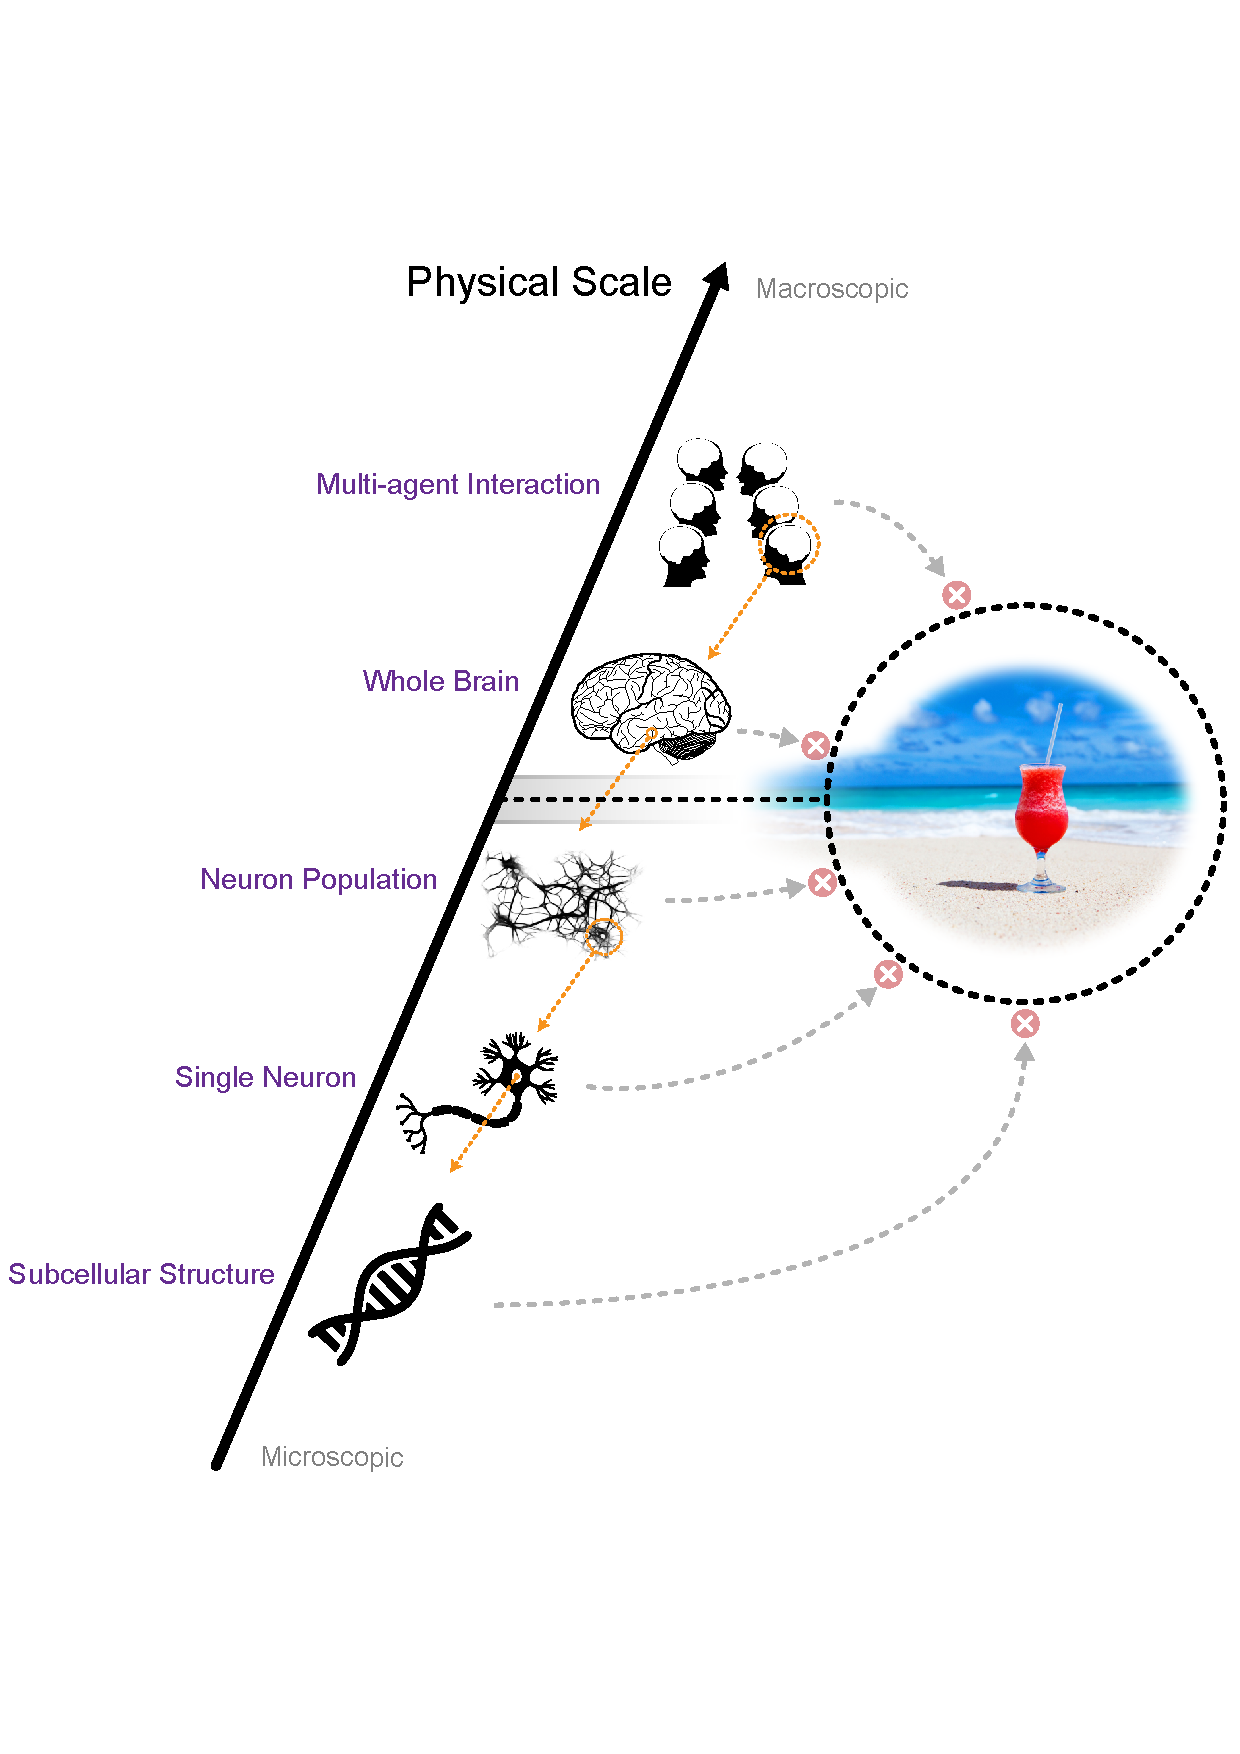
\includegraphics[width=\textwidth]{WritingMaterials/Fig_ScaleProblemOfConsciousness/ScaleProblemOfConsciousness.pdf}
			\caption{The scale problem of consciousness: Human conscious experience does not reflect information from every scale. Only information at a certain coarse-grained scale in the neural system is reflected in consciousness.}
			\label{fig:scaleproblem}
	   	\end{figure}


% ============================================================================ %
%                       Non-trivial informational closure                      %
% ============================================================================ %
	\section{Non-trivial Informational Closure} \label{sec:Non-trivial informational closure}
		The notion of non-trivial informational closure (NTIC) is introduced by \cite{BERTSCHINGER.2006}. The concept of closure is closely related to system identification in systems theory. One can distinguish a system from its environment by computing the closedness of the system \citep{maturana1991autopoiesis, rosen1991life, pattee2012evolving, luhmann1995probleme}. The closedness can be further quantified by information theory.



		% Definition of informational closure
			\linelabel{line:r1q1a}Consider two processes, the environment process $(E_t)_{t \in \mathbb{N}}$ and the system's process $(Y_t)_{t \in \mathbb{N}}$ and let their interaction be described by the Bayesian network in Fig.~\ref{fig:SystemAndEnv}. Then, information flow $J_{t}$ from the environment $E$ to a system $S$ at time $t$ can be defined as the conditional mutual information $I$ between the current environment state $E_{t}$  and the future system state $Y_{t+1}$ given the current system state $Y_{t}$

				\begin{equation}
    				\label{eq:InformationFlow}
    				\left.\begin{array}
    				{rl}{J_{t}(E \rightarrow Y )} & {:= I(Y_{t+1};E_{t}|Y_{t})} \\
    				{ } & { \ = I(Y_{t+1};E_{t}) - (I(Y_{t+1};Y_{t})-I(Y_{t+1};Y_{t}|E_{t}))}
    				\end{array}\right.
				\end{equation}

            
				\begin{figure}
					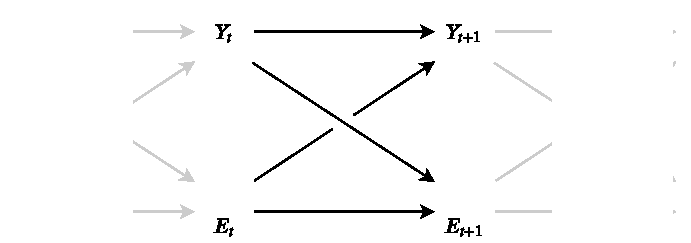
\includegraphics[width=\textwidth]{WritingMaterials/Fig_SystemAndEnv/SystemAndEnv_2.pdf}
					\caption{The dependencies between a system and its environment.} % Figure adapted from \cite{BERTSCHINGER.2006}
					\label{fig:SystemAndEnv}
				\end{figure}


			\noindent
			\cite{BERTSCHINGER.2006} defines that a system is informationally closed when information flow from the environment to the system is zero.

				\begin{equation}
				J_{t}(E \rightarrow Y )=0
				\label{eq:informationflow2}
				\end{equation}


			% ------------------------------- trivial case ------------------------------- %
			\noindent
			Information closure (minimising $J_t$) is trivial if the environment and the system are entirely independent of each other.

				\begin{equation}
				\begin{aligned}
				{I(Y_{t+1};E_{t})=0}&&{\Rightarrow}&&{J_{t}(E \rightarrow Y )=0}
				\end{aligned}
				\end{equation}


			% -------------------------------- non-trivial ------------------------------- %
			\noindent
			However, informational closure can be formed non-trivially. In the non-trivial case, even though a system contains (or encodes) information about the environmental dynamics, the system can still be informationally closed. In such cases, the mutual information between the current states of the environment and the future state of the system is larger than zero.

				\begin{equation}
				I(Y_{t+1};E_{t}) > 0
				\end{equation}

			\noindent
			This also implies
				\begin{equation}
					I(Y_{t+1};Y_{t})-I(Y_{t+1};Y_{t}|E_{t}) > 0
				\end{equation}



			\noindent
			And, non-trivial informational closure can be defined as
				\begin{align}
%				\label{eq:NTIC}
    				% \left.\begin{array}
    				NTIC_t(E\rightarrow Y) :&=I(Y_{t+1};Y_{t})-I(Y_{t+1};Y_{t}|E_{t}) 
    				\label{eq:NTIC1}\\
    				&=I(Y_{t+1};E_{t})-I(Y_{t+1};E_{t}|Y_{t}) 
    				\label{eq:NTIC2}
    				% \end{array} \right.
				\end{align}
			

			\noindent
			Hence, maximising $NTIC_t(E\rightarrow Y)$ amounts to
				\begin{equation}
    				\label{eq:nticObjective}
    				\begin{aligned}
    				& \text{maximising} & { } & I(Y_{t+1};Y_{t}) & { } & \text{and} \\
    				& \text{minimising} & { } & I(Y_{t+1};Y_{t}|E_{t}) & { }
    				\end{aligned}
				\end{equation}
			
			\noindent
			One can also maximise $NTIC_t(E\rightarrow Y)$ by 
				\begin{equation}
    				\label{eq:nticObjective2}
    				\begin{aligned}
    				& \text{maximising} & { } & I(Y_{t+1};E_{t}) & { } & \text{and} \\
    				& \text{minimising} & { } & I(Y_{t+1};E_{t}|Y_{t}) & { }
    				\end{aligned}
				\end{equation}			

			\noindent
			This implies the system contains in itself all the information about its own future and the self-predictive information contains the information about the environment. Therefore, to form NTIC, the system can internalise and synchronise with the dynamics of the environment, e.g., model the environment. Furthermore, having high degrees of NTIC entails having high predictive power about the environment. This gives biological agents a great functional and evolutionary advantage. 
			

% ============================================================================ %
%                            Neural coarse-graining                            %
% ============================================================================ %
	\section{Coarse-graining in the Neural System} \label{sec:Neural coarse-graining}

		%% stochasticity at microscopic levels
		The formation of NTIC with a  highly stochastic process is challenging. NTIC requires the predictability of the system state and is therefore impeded by noise in the system. Information processing at the microscopic levels (the cellular levels) in neural systems suffers from multiple environmental noise sources such as sensor, cellular, electrical, and synaptic noises. For example, neurons exhibit large trial-to-trial variability at the cellular level, and are subject to thermal fluctuations and other physical noises \citep{faisal2008noise}. 
		
  
        %% Our argument
		However, it is possible that neural systems form NTIC at certain macroscopic levels through coarse-graining of microscopic neural states. Coarse-graining refers to many-to-one or one-to-one maps which aggregate microscopic states to a macroscopic state. In other words, a number of different micro-states correspond to the same value of the macro-variable \citep{price2007causation}. Coarse-grainings, can therefore form more stable and deterministic state transitions and more often form NTIC processes. For neural systems this means that a microscopically noisy neural system may still give rise to an NTIC process on a more macroscopic scale.
		
		Indeed, empirical evidence suggests that coarse-graining is a common coding strategy to establish robustness against noise at microscopic levels of the neural system. For instance, the inter-spike intervals of an individual neuron are stochastic. This implies that the state of an individual neuron does not represent stable information. However, the firing rate, i.e. the average spike counts over a given time interval, is more stable and robust against noise such as the variability in inter-spike intervals. Using this temporal coarse-graining strategy, known as rate coding \citep{adrian1926impulses, gerstner2002spiking, maass2001pulsed, panzeri2015neural, stein2005neuronal}, neurons can encode stimulus intensity by increasing or decreasing the firing rate \citep{kandel2000principles}. \citep{stein2005neuronal}. The robustness of the rate coding is a direct consequence of the many to one mapping (i.e., coarse-graining).
		
		% population code
		Population coding is another example of encoding information through coarse-graining in neural systems. In this coding scheme, information is encoded by activation patterns of a set of neurons (a neuron population). In the population coding scheme, many states for a neuron population map to the same state of macroscopic variables which encode particular informational contents, thereby reducing the influence of noise in individual neurons. That is, stable representations can be formed through coarse-graining the high dimensional state space of a neuron population to a lower dimensional macroscopic state space \citep{kristan1997population, pouget2000information, binder2009encyclopedia, QuianQuiroga2009}. Therefore, individual neuron states (the microscopic level) are not informative enough about the complete encoded contents at the population level (the macroscopic level). Instead, coarse-grained variables are better substrates for stably encoding information and allow the neural system to ignore noisy interactions at the fine-grained level \citep{Woodward2007-WOOCWA}.
		
        These two examples show that the known coding schemes can be viewed as coarse-graining, and provide stochastic neural systems with the ability to form more stable and deterministic macroscopic processes for encoding and processing information reliably. We argue that through coarse-graining the neural systems is able to form NTIC processes at macroscopic levels. Based on the merit of coarse-graining in neural systems, we propose a new theory of consciousness in the next section. 



% ============================================================================ %
%               A neural coarse graining theory of consciousness               %
% ============================================================================ %
	\section{\acf{OurTheory}}\label{sec:OurTheory}
	
        In this section, we propose a new theoretical framework of consciousness: \acf{OurTheory}. The main hypothesis is that conscious processes are captured by what we call \textit{C-processes}. We first define C-processes, then state our hypothesis and discuss its implications.
        
        
		\begin{figure}[H]
		    \centering
			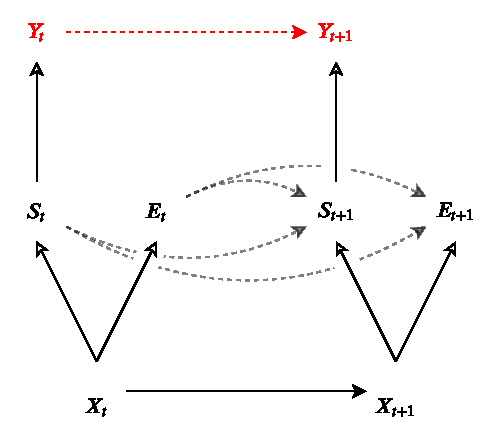
\includegraphics[width=\textwidth]{WritingMaterials/Fig_FullGraph/FullGraph.pdf}
			\caption{The information flow amounts the universe $X$, the system $S$, the environment of the system $E$, and the coarse-grained process $Y$ of the system $S$. The solid line with a filled arrow from $X_t$ to $X_{t+1}$ represents the microscopic dynamic of the universe. The solid lines with a empty arrow represent directions of coarse-graining. The dashed lines represents virtual dependencies between  two macroscopic variables. The red $Y_t$, $Y_{t+1}$, and the red dashed line in between represents a macroscopic process which forms informational closure at a certain coarse-grained level.}
			\label{fig:fullgraph}
	   	\end{figure}

	   	% ------------------------------- definition 1 ------------------------------- %
	   	In order to define C-processes we need to define coarse-grainings first. Every coarse-graining is characterised by a function that maps the microscopic process to the coarse-grained macroscopic process. More formally: 
	   	
	   	\begin{definition}
	   	\linelabel{line:r2q1-1} Given a stochastic process $X$ with state space $\mathcal{X}$, a \emph{coarse-graining of $X$} is a stochastic process $Y$ with state space $\mathcal{Y}$ such that there exists a function \footnote{Functions in the mathematical sense used here are always either one-to-one or many-to-one.} $f_Y:\mathcal{X}\rightarrow \mathcal{Y}$ with $Y_t=f_Y(X_t)$.  
	   	\end{definition}
	   	A more general definition of coarse-grainings that maps temporally extended sequences of the microscopic process to macroscopic states are possible but for this first exposure of our theory the simpler definition above is sufficient. 
	   	
	   	% ------------------------------- definition 2 ------------------------------- %
        \begin{definition}
        Given a stochastic process $X$ called the universe process, a \emph{C-process} is a coarse-graining $Y$ of $X$ such that the following two conditions are satisfied (see Fig.~\ref{fig:fullgraph}):
        \begin{enumerate}
        \item $Y$ is informationally closed to $X$
        \item there exists a pair $(S,E)$ of coarse-grainings of $X$ such that 
        \begin{itemize}
            \item $Y$ is a coarse-graining of $S$,
            \item the state space $\mathcal{X}$ of $X$ is equal to the Cartesian product of the state spaces $\mathcal{S}$ and $\mathcal{E}$ of processes $S$ and $E$ respectively, formally $\mathcal{X}=\mathcal{S}\times\mathcal{E}$, and 
            \item $Y$ is NTIC to $E$, formally:
        \begin{align}
            NTIC_t(E\rightarrow Y) >0
        \end{align}
        \end{itemize} 
        \end{enumerate}
       \end{definition}
                               
        \linelabel{line:IC2CG}
        With the two definitions we can state the main hypothesis of \ac{OurTheory}
        \footnote{Note that, here we applied the same definitions of information flow (Eq.~\ref{eq:InformationFlow}) and informational closure (Eq.~\ref{eq:informationflow2}) to the system-environment dependency (e.g. $J_{t}(E \rightarrow Y )=0$) and the micro-macro level dependency (e.g. $J_{t}(X \rightarrow Y )=0$), even though the Bayesian graphs are different between the two scenarios. This follows the common settings in previous studies (e.g. \cite{BERTSCHINGER.2006, PFANTE.2014}).}:
        
        \begin{hypothesis}
        A process $Y$ is conscious if and only if it is a C-process of some process $X$. Also the content of consciousness $C_t^{Content}$ at time $t$ is the state $y_t$ of the C-process at time $t$ and the level of consciousness $C_t^{Level}$ is the degree of NTIC of the C-process to the environment i.e. $NTIC_t(E\rightarrow Y)$:
        \begin{align}
            C_t^{Content} &= y_t \label{eq:cContent}\\
            C_t^{Level} &= NTIC_t(E\rightarrow Y) \label{eq:cLevel}
        \end{align}
        \end{hypothesis}
        
        A concrete example in the context of neuroscience is that $X$ represents the microscopic level of the universe, $S$ a cellular level process in the neural system, $Y$ a more macroscopic process of the neural system coarse-grained from the cellular level process $S$, and $E$ the environment which the cellular level process $S$ interacts with. \linelabel{line:neu-env} The environment $E$ may include other processes in the neural system, the sensors for perception and interoception, and external physical worlds.\\
        
        Based on the hypothesis, \ac{OurTheory} leads to five core implications: 
        \begin{description}
            \item[Implication 1.] 
            Consciousness is information. Here, "informative" refers to the resolution of uncertainty. Being in a certain conscious state rules out other possible conscious states. Therefore, every conscious percept resolves some amount of uncertainty and provides information. \\ 
            This implication is also in agreement with the "axiom" of \textit{information} in Integrated Information Theory (IIT 3.0) which claims that \textquote[{\citealp[P.~2]{oizumi2014phenomenology}}]{...an experience of pure darkness is what it is by differing, in its particular way, from an immense number of other possible experiences...}
            
            \item[Implication 2.] 
            Consciousness is associated with physical substrates and the self-information of the conscious percept is equal to the self-information of the corresponding physical event. This is a direct implication from our hypothesis that every conscious percept $C_t^{Content}$ corresponds to a physical event $y_t$. 
            
            %In \ac{OurTheory}, we consider information is the common language between conscious experience and the physical reality. This means that consciousness is fundamentally associated with information \citep{chalmers1996conscious, tononi2004information, gamez2011information, Gamez2016}).
            
            \item[Implication 3.] 
            Conscious processes are self-determining. This is a direct implication of the requirement that $Y$ is informationally closed with respect to $X$. To be informationally closed with respect to $X$, no coarse-graining knows anything about the conscious process' future that the conscious process does not know itself. This self-determining characteristics is also in line with our daily life conscious experience which often shows stability and continuity and is ignorant of the stochasticity (e.g., noise) of the cellular levels.
            

            
            \item[Implication 4.] 
            Conscious processes encode the environmental influence on itself. This is due to the non-triviality of the informational closure of $Y$ to $E$. At the same time all of this information is known to the conscious processes themselves since they are informationally closed with respect to their environments. This also suggests that conscious processes can model the environmental influence without knowing more information from the environment.
            
            \item[Implication 5.]
            Conscious processes can encode environmental information (by forming NTIC), however, be ignorant to part of the information of more microscopic processes (from Implication 3 and 4). This is in line with our conscious experience that information that every conscious percept provides represent rich and structured environmental states without involving all the information about microscopic activities.
        \end{description}
		
		
		% ---------------------------------------------------------------------------- %
        %        Level of Consciousness correlates degrees of NTIC of a process        %
        % ---------------------------------------------------------------------------- %
	    \subsection{Level of Consciousness is Equal to the Degree of NTIC of a Process}\label{sec:cl}
            According to Eq.~\ref{eq:nticObjective}, \ac{OurTheory} implies that conscious levels are determined by two quantities. 
            
            First, to form a high level of NTIC, one can increase the mutual information $I(Y_{t+1};Y_{t})$ between the current internal state $Y_t$ and the future internal state $Y_{t+1}$. In other words, conscious levels are associated with the degree of self-predictive information \citep{bialek2001predictability}. This mutual information term can be further decomposed to two information entropy quantities: 
            
            \begin{equation}
            \label{eq:SelfEntropy}
            I(Y_{t+1};Y_{t}) = H(Y_{t+1}) - H(Y_{t+1}|Y_t)
            \end{equation}
            
            This implies that a highly NTIC process must have rich dynamics with self-predictability over time. Another implication is that complex systems can potentially attain higher levels of consciousness due to the larger information capacities needed to attain high mutual information. This outcome is consistent with the common intuition that conscious levels are often associated with the degree of complexity of a system.
    
    	    Second, one can minimise the conditional mutual information $I(Y_{t+1};Y_{t}|E_{t})$ to increase the level of NTIC. This quantity suggests that conscious level increases with the amount of information about the environment state $E_t$ that the NTIC process encodes in its own state $Y_t$. In other words, $Y_t$ should not contain more information about $Y_{t+1}$ than $E_t$. An important implication is that agents interacting with a complex environment have the chance to build a higher level of NTIC within their systems than those living in a simple environment. In other words, the level of consciousness is associated with environmental complexity. 
    	   
    	    %% not monotonic
    		\linelabel{line:non-monotonic}It is important to note that NTIC can be a non-monotonic function of the scale of coarse-graining\footnote{We have known that NTIC is not a non-monotonic function of the scale of coarse-graining. However, we currently have limited understanding about this relationship. Future work is needed and may involve relevant informational techniques (e.g.,partial information decomposition).}. At the finest scale, when we consider the dynamics of the whole universe as a process, the universe should be an informationally closed. However, there exists no environment to the universe and, therefore, NTIC of the universe is zero (trivially closed). On the other hand, overly coarse-grained macroscopic variables  also result in low values of NTIC. For example, in an extreme scenario, when all microscopic states map to a single macroscopic variable, the macroscopic level does not have any informational capacity and thus cannot have  mutual information between adjacent time steps.  Therefor, processes at certain levels of coarse-graining in the neural system can form high degrees of NTIC (Fig.~\ref{fig:LevelOfConsciousness}). \ac{OurTheory} indicates that human consciousness occurs at the level of coarse-graining where higher NTIC is formed within the neural system. 
    		
    		\begin{figure}[H]				
        		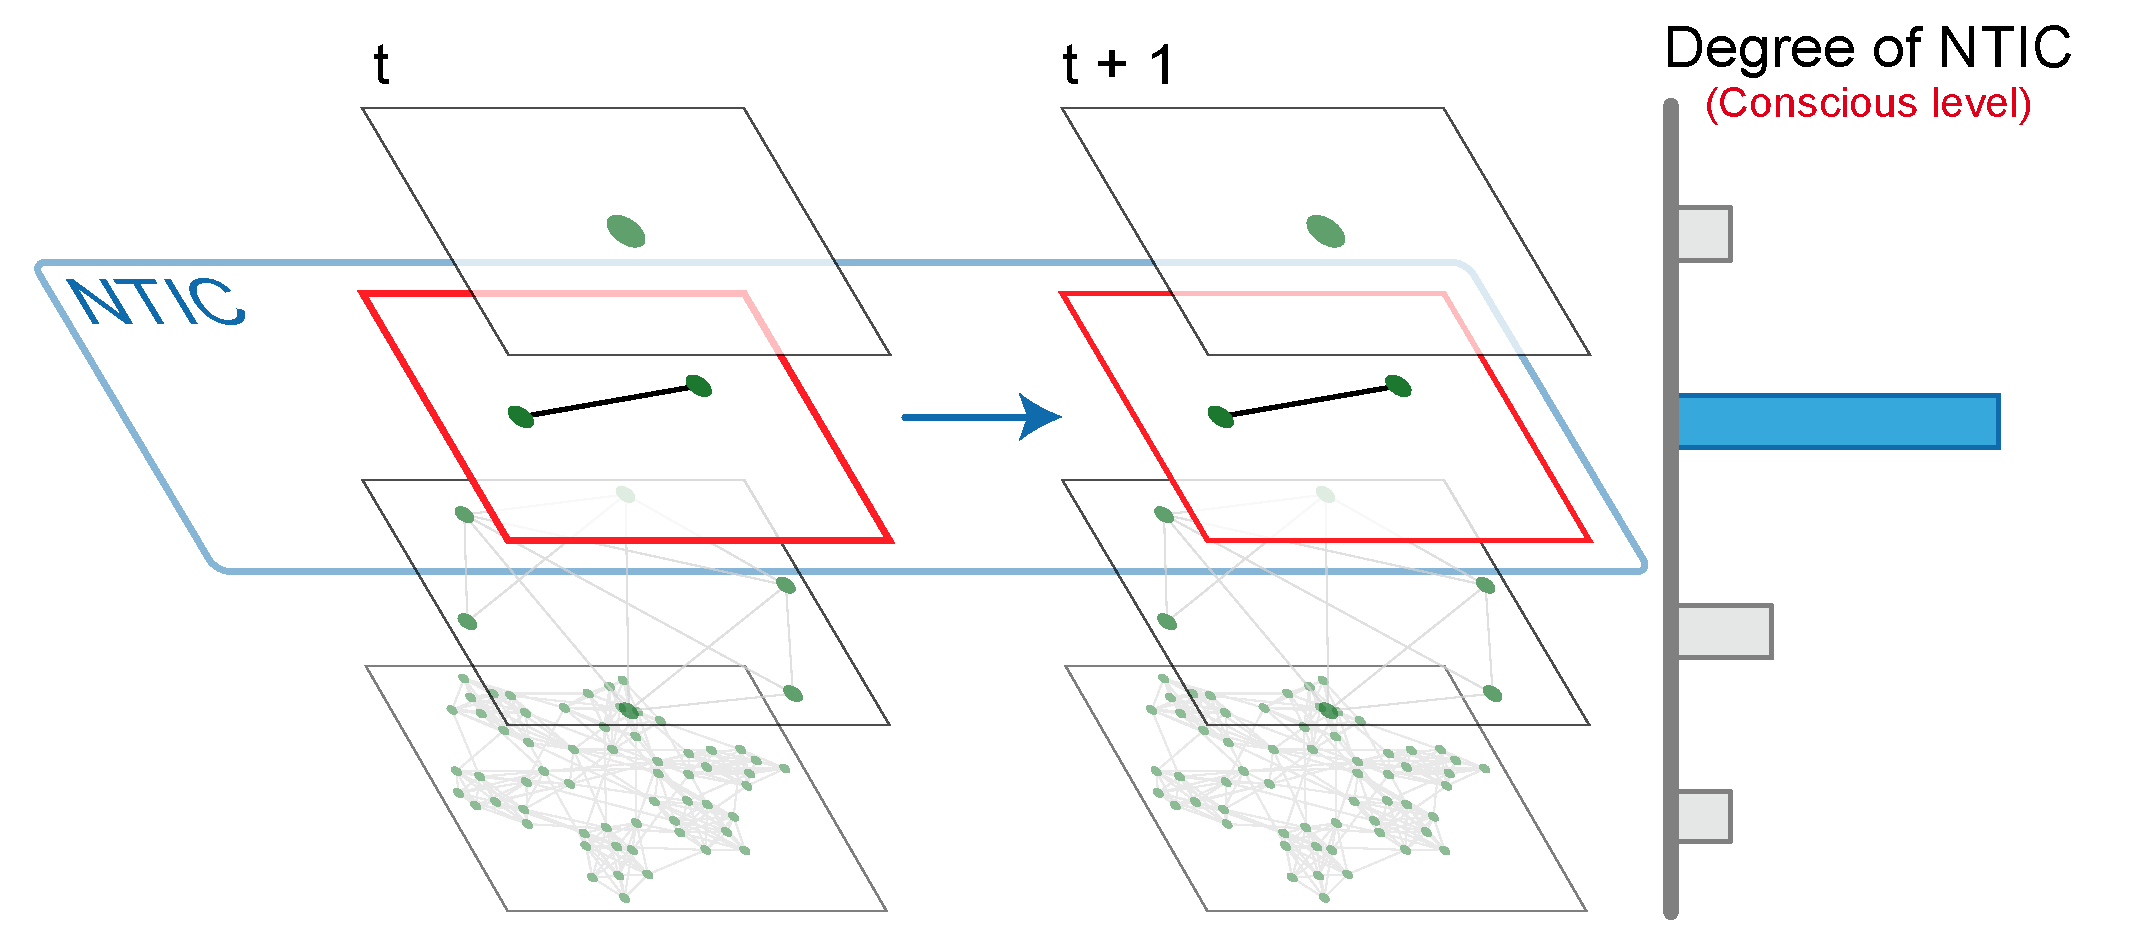
\includegraphics[width=\textwidth]{WritingMaterials/Fig_nonMono/nonMono.pdf}
        		\caption{A non-monotonic relationship between Level of coarse-graining and level of consciousness.}
        		\label{fig:LevelOfConsciousness}
    		\end{figure}
            
    			
		\subsection{Conscious Contents Corresponding to States of a NTIC Process}\label{sec:cc}
    	    % richness 
    		\ac{OurTheory} proposes that conscious contents correspond to the states of NTIC processes (Eq.~\ref{eq:cContent}). This implies that the size of the state space of an NTIC process is associated with the richness of conscious contents that the process can potentially have. Therefore, a complex NTIC process with a high dimensional state space can have richer conscious experience than a simple NTIC process can have. This outcome is consistent with the intuition that the richness of conscious contents is associated with the complexity of a system. 
    		
    		% CC doesn't include all microscopic states
    		As mentioned above, informational closure can happen between scales of coarse-graining within a single system. Thus, a macroscopic NTIC process can be ignorant to its microscopic states. \ac{OurTheory} argues that human conscious contents do not reflect cellular level activity because the conscious process which corresponds to a macroscopic NTIC process is informationally closed to the cellular level in the human neural system. Further more, since NTIC processes are informationally closed, each of them can be considered as a reality. In the extreme case, when the information flow from its microscopic processes and environment to the informationally closed process is completely zero (Eq.~\ref{eq:informationflow2}), the future states of the process is only determined by its past states. 
    		
    		\linelabel{line:encode}Importantly, NTIC processes internalise the environmental dynamics in its states \citep[also see P.~4][]{BERTSCHINGER.2006}. This suggests that a NTIC process can be considered as a process that models the environmental dynamics.This implication fits well with some theories of consciousness (for example, world simulation metaphor ~\citep{revonsuo2006inner}). Note that \ac{OurTheory} doesn't assume that generative models are necessary for consciousness. The implication is a natural result of processes with NTIC. 
            
            Finally, a coarse-graining can be a many to one map from microscopic to macroscopic states and \ac{OurTheory} proposes that conscious contents $C^{Content}$ is the state of the NTIC process $Y$. Therefore, \ac{OurTheory} implies multiple realisation thesis of consciousness \citep{putnam1967psychological,bechtel1999multiple} which suggests that different physical implementations could map to the same conscious experience.
            
            
		% ---------------------------------------------------------------------------- %
        %             Reconciling the levels and contents of consciousness             %
        % ---------------------------------------------------------------------------- %
	    \subsection{Reconciling the Levels and Contents of Consciousness}\label{sec:reconcile}
    	    While it is useful to distinguish the notion of the levels and contents of consciousness, whether they can be clearly dissociated has been a matter of debate \citep{bayne2016there, Fazekas2016}. In \ac{OurTheory}, conscious levels and conscious contents are just two different properties of NTIC processes, and, therefore, naturally reconciles the two aspects of consciousness. In an NTIC process with a large state space, conscious contents should also consist of rich and high dimensional information. Therefore, this framework integrates the levels and the contents of consciousness in a coherent fashion by providing explicit formal definitions of the two notions.  
    	    
    	    
    	    According to Sec.~\ref{sec:cl} and Sec.~\ref{sec:cc}, an important implication from \ac{OurTheory} is that both conscious levels and conscious contents are associated with the state space of an NTIC process $Y$. A large state space of $Y$ contributes conscious levels through the mutual information $I(Y_{t+1};Y_{t})$ and also contributes richer conscious contents by providing more possible states of conscious processes. 
    	    \ac{OurTheory} therefore explains why, in normal physiological states, conscious levels and conscious contents are often positively correlated \citep{laureys2005neural}. This implication is also in line with the intuition in which consciousness is often associated with complex systems.
    			
            % ---------------------------------------------------------------------------- %
            %                              Dynamical Boundary                              %
            % ---------------------------------------------------------------------------- %
            % \subsection{Dynamical Boundary}
            % Our theory predicts that the boundary of a conscious system is dynamical. The boundary is determined by the NTIC process. This implies that when the structure of interaction between variables changes the physical boundaries supporting consciousness should also change. If some coarse-grained variables encode environmental information, they may become necessary components to form high NTIC. In such case, these coarse-grained variables are "recruited" inside the boundary of conscious processes. Note that, due to synergistic information, even recruiting some new variables may largely increase the level of NTIC. 
            % This may explain why consciousness is tightly associated with binding and integration of information in human perception and cognition. Another crucial implication is that the same neural substrates may not be always involved in conscious processing rather it depends on whether it creates high NTIC with other members in the neural system. \needfig{Maybe I need a figure here as well}
    
    
    % ============================================================================ %
    %                    Conscious versus Unconscious Processing                   %
    % ============================================================================ %
	\section{Conscious Versus Unconscious Processing}\label{sec:Conscious versus Unconscious Processing}
	    In this section, we show how \ac{OurTheory} can explain and make predictions about what processes are conscious and what are unconscious. \ac{OurTheory} is constructed using information theory. Therefore, \ac{OurTheory} can provide predictions based on the mathematical definitions. 
		
        % ---------------------------------------------------------------------------- %
        %                            Unconscious Processing                            %
        % ---------------------------------------------------------------------------- %
        \subsection{Unconscious Processing}
            Regarding unconscious processing, we highlight two scenarios in which the degree of NTIC is rendered low for a process, and thereby making the process less conscious.
        
            \subsubsection*{Processes that are not Informationally Closed}\label{sec:reflexive}
            ICT leads to some surprisingly simple conscious processes. Consider the case already noted by \citet{BERTSCHINGER.2006} where the environment process is deterministic (or close to it) and the system just copies the environment process. Then the system achieves a high value of NTIC with respect to the environment. ICT states that such processes are conscious. 
            
            (We assume Transfer entropy from environment to system is equal to transfer entropy from sensor to system by definition).
            
            However, in more realistic cases the system cannot copy the environment state because it observes only part of it. 
            % and/or because it is itself not large enough to contain a copy of the environment. 
            
            Let us assume that the system only observes a part of the (still environment state.
            \footnote{In theory this part of the environment state may still evolve deterministically over time in which case the system need only copy this part to achieve NTIC and consciousness. This seems to be a rare case as well and we assume the observed part of the environment is not close to deterministic in the following.} 
            In this case it is well known that the observed part of the environment need not even be a Markov process even if the environment itself is deterministic. So the mutual information between subsequent observations may be much lower than the mutual information between subsequent environment states.
            
            Furthermore, in this case the transfer entropy from environment to the system becomes equal to the transfer entropy from the observed part of the environment to the system. 
            
            Finally, note that the transfer entropy that can be achieved by copying the environment state or the observed part of the environment state is bounded from above by the mutual information between the subsequent environment states or observations. Copying the environment state corresponds to setting $S_{t+1}=E_t$ such that the transfer entropy is
            \begin{align}
             I(S_{t+1}:E_t|S_t)=I(E_t:E_t|E_{t-1})=H(E_t|E_{t-1}).
            \end{align}
            We can represent the part of the environment that we observe by the value of a function applied to the environment state so that
            
            
            
            
            
            
            % In such situations ITC predicts that higher levels of consciousness are achieved if the system can anticipate the next observed values which requires a higher internal self-determination than that of the copies of the observations.
            
            % Another way to put this is the higher the difference in predictability of the sensor values and the entrie environment state the more potential is there to increase the level of consciousness for the system by modelling the underlying hidden Markov process i.e.\ environment.
            
            % Also assume that the part that the system observes is not itself deterministic or close to it but that the underlying environment is. 
            
            % A system with a high NTIC in such situations must 
            % Then the system can decrease the transfer entropy from the environment to itself by anticipating the next observation. This is due to the fact that the transfer entropy from the environment to the system is equal to the transfer entropy from the observations to the system.
            
            
            
            
            
            % does not have access to the entire environment state and instead observes only part of it. This part is rarely close to deterministic even if the entire environment is deterministic. In order to achieve informational closure with respect to the entire environment the system has to achieve closure exactly with respect to its sensor values.  
            
            
            % we could copy it to get closure. In realistic situations we are not sure whether the environment is informationally closed but even if we assume it is we can confidently assert that we don't observe it completely and that the part we do observe (our sensory values) are not themselves closed. For example, the images on our retina are insufficient to predict their successors without imagining the outside world behind them. This imagining however requires internal processing like recurrent connections.
           		
                The higher the transfer entropy from environment to the system the lower NTIC (Eq.~\ref{eq:nticObjective2}) and therefore, according to ICT, the lower the level of consciousness. Under the assumptions above, 
                
                high transfer entropies occur when the current state of a process depends primarily on the environment state (see Fig.~\ref{fig:reflexive}), but receives little influence from its past state. Reflexive behaviours \citep{casali2013theoretically} can be considered an example of this scenario. In \ac{OurTheory}, if we can view reflexive behaviours as situations in which the internal state $Y_t$, which triggers reflexive action, is determined by the environment state $E_{t-1}$ overruling the influences from its own past $Y_{t-1}$.  Such interpretation of reflexive behaviour from the viewpoint of \ac{OurTheory} naturally explains why reflexes do not involve conscious experience of external stimuli. 

             	% reflexive behaviour
        		\begin{figure}[H]
        			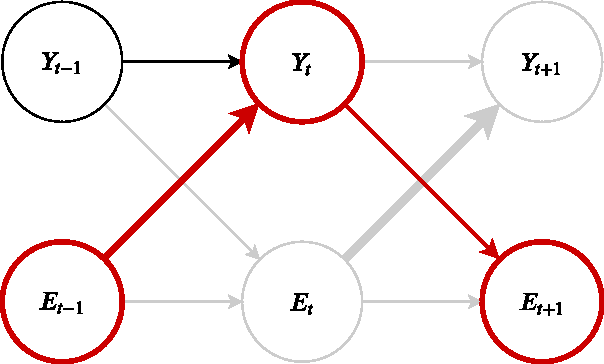
\includegraphics[width=0.8\textwidth]{WritingMaterials/Fig_Reflexive/Reflexive.pdf}
        			\caption{
        			    A diagram depicting the information flow in reflexive behaviours (shown by the red nodes and arrows) happening through the interaction between a process $Y$ and its environment $E$. In such situations, the internal state $Y_t$ is mostly dependent on the environment state $E_{t-1}$ but less on its past state $Y_{t-1}$. Therefore, the process $Y$ is not informational closed. As a  consequence, $Y$ is unable to form high NTIC and, therefore, remain less conscious or unconscious. 
        			    }
        			\label{fig:reflexive}
        		\end{figure}  
        		
        		The same principle can be applied to interpret blindsight \citep{humphrey1999history, humphrey1974vision, Humphrey1970} and procedural memory \citep{doyon2009contributions, ashby2010cortical} which are often considered as unconscious processes.
        		\linelabel{line:r2q6}Blindsight patients are able to track objects, avoid obstacles, and make above chance-level visual judgements with degraded or missing visual experience (however, in some cases, they may still preserve some forms of conscious experience, see \cite{overgaard2011visual, mazzi2016blind}). We argue that action outputs of blindsight can be directly guided by sensory inputs through stimulus-response maps. The neural circuits are not informationally closed and, therefore, unconscious. Similarly, for procedural memory, the state transitions of action controls largely depends on the concurrent environmental states. This prevents the internal processes of procedure memory from informational closure and being conscious. \ac{OurTheory} also offer an interpretation as to why patients with visual apperceptive agnosia \citep{james2003ventral} can perform online motor controls without visual awareness of action targets \citep{10.3389/fneur.2014.00255}. 

        		As we have seen in the examples above, a crucial implication of \ac{OurTheory} is that a pure feedforward network cannot produce consciousness because NTIC requires a form of memory $I(Y_{t+1};Y_{t})$. Without memory, a network's current state is entirely driven by the input the network receives from the environment without any influence from its own past states. Therefore, such a network is incapable of forming an NTIC. In contrast, a network with recurrent loops can maintain information about its own past states. This forms an information channel between the past and the future states of the network and, thus, makes the network capable of being informationally closed. This result coincides with theories of consciousness emphasising the importance of recurrent circuits to consciousness \citep{lamme2006towards, edelman1992bright, tononi2008neural}.

            \subsubsection*{Processes are Trivial closed}
                According to \ac{OurTheory}, when encoded information in a process is trivial, i.e. no mutual information between the process states and its environment states $I(Y_{t+1};E_{t})$ (Eq.~\ref{eq:nticObjective2}), this could lead low NTIC. In such case, this process is considered to be unconscious due to the low level of NTIC. This implies an isolated process which is simply informationally closed is insufficient to be conscious. 
                This mathematical property of \ac{OurTheory} provides a natural and intuitive (but only partial, see the current challenge in  Sec.~\ref{sec:Limitation and Future work}) solution to the boundary and the individuality problem of consciousness
                    \footnote{The boundary problem of consciousness refers to identifying physical boundaries of conscious processes and the individuality problem of consciousness refers to identifying individual consciousnesses in the universe.}
                \citep{Raymont2006-RAYUOC}. Consider a NTIC process $Y$ and an isolated informationally closed process $\hat{Y}$ with only trivial information. Adding $\hat{Y}$ to $Y$ can still keep informational closure, but, however, does not increase non-trivial information, i.e. doesn't affect consciousness. 
                
    			\begin{equation}
    			    \begin{aligned}
                        I(Y,\hat{Y};E) & = H(Y,\hat{Y}) - H(Y,\hat{Y}|E) \\
                                       & = H(Y) + H(\hat{Y}|Y) - (H(Y|E)+H(\hat{Y}|Y,E)) \\
                                       & = H(Y) + H(\hat{Y}) - (H(Y|E)+H(\hat{Y})) \\
                                       & = H(Y) - H(Y|E)\\
                                       & = I(Y;E)				
    				\end{aligned}
    			\end{equation}
                
                This implies that isolated processes with trivial information do not contribute consciousness and should be considered being outside the information boundary of the conscious processing (for more details of the boundary detection procedure, see \cite{krakauer2014information}). 
                This property also implies that consciousnesses do not emerge from just aggregating informationally closed (isolated) processes which contain trivial information.%\footnote{However, we do not exclude the possibility that triviality of encoded information is just a proxy of other quantities which more directly associate with consciousness. We point out that this is a limitation of the current version of \ac{OurTheory} in Sec.~\ref{sec:Limitation and Future work}.}
                
                
                



        % ---------------------------------------------------------------------------- %
        %                             Conscious Processing                             %
        % ---------------------------------------------------------------------------- %
		\subsection{Conscious Processing}\label{sec:conscious processing}
		    According to \ac{OurTheory}, we claim that any process, system, or cognitive function which involves any NTIC process should be accompanied by conscious experience. 
		    
		    Previous consciousness research has identified a number of diverse cognitive processes often accompanied by conscious experience. \ac{OurTheory} provides an integrated account for the reason why these processes involve conscious experience. As mentioned above, an NTIC process can be seen as an internal simulation engine for the agent-environmental interactions \citep{BERTSCHINGER.2006}. Therefore, information encoded in NTIC processes is essential for several cognitive processes. 
		    
		    One of the most valuable information is the predictions about the environmental states. Cognitive functions requiring agent-scale environmental predictions are likely to recruit NTIC processes and therefore accompanied by conscious experience, for example planning and achieving long term goals.
		   
            Second, as a simulation engine, with a given initial state, an NTIC process can self-evolve and simulate the environmental transitions. Cognitive functions involving simulations are expected to involve NTIC processes. Consequently, mental simulation, imagination, computing alternative realities, and generating counterfactuals often come with conscious experience. 
            
    	    Third, as an informationally closed system, an NTIC process can still provide environmental information without new sensory inputs. This is crucial for many types of off-line processing. Therefore, in contrast to reflexive-like behaviours mentioned above (Sec.~\ref{sec:reflexive}), behaviours requiring off-line computations \citep{milner1999paradoxical, himmelbach2005dorsal,revol2003pointing} often involve conscious experience. 
    	    
    	    Finally, for agents adapting to complex environments (e.g., human being), any state of the NTIC process can be seen as an integration of high dimensional information. To accurately encode information about the complex environmental states and transitions, the NTIC process requires knowledge about the complex causal dependencies involved in the environment. Therefore, cognitive functions requiring large scale integration are likely to involve NTIC processes and accompanied by conscious experience. % Furthermore, the high dimensional integrated information is also critical for an agent to learn new behaviours to achieve flexibility and the strategic behavioural controls and decision-making. 
    	    
    	    Note that many of the claims above are compatible with several theories of consciousness which highlight the connection between consciousness and internal simulation, predictive mechanism, or generative models inside a system (e.g. world simulation metaphor ~\citep{revonsuo2006inner}, predictive processing and Bayesian brain~\citep{clark_2013,Hohwy2013,seth2014predictive}, generative model and information generation~\citep{kanai_chang_yu_de_abril_biehl_guttenberg_2019}). Instead of relating functional or mechanistic aspects of a system to consciousness, \ac{OurTheory} captures common informational properties underlying those cognitive functions associated with consciousness. As such, \ac{OurTheory} does not assume any functionalist perspective of consciousness, which associate specific functions to consciousness.  That is to say, since \ac{OurTheory} associates information  with consciousness, functional features accompanied by consciousness are collateral consequences of neural systems utilising NTIC processes for adaptive functions. 
    	    
    	    In sum, we argue that cognitive functions involving the NTIC process are inevitably accompanied by consciousness. Having an NTIC process is potentially an effective approach to increase fitness in the evolution. It is likely that biological creatures evolve NTIC processes at some point in the evolution. Due to the fundamental relation between information and consciousness, biological creatures also evolve different degrees of consciousness depending on the physical scales and the complexity of the environments they adapt to. 
    	    
    	    \ac{OurTheory} starts with a non-functional hypothesis, however, it accounts for the association between  functional and consciousness. \ac{OurTheory} further demonstrates remarkable explanatory power for various findings of conscious and unconscious processing. 
	    
    % % ============================================================================ %
    % %                        Comparison with other theories                        %
    % % ============================================================================ %
    \section{Comparison with Other Relevant Theories of Consciousness}\label{sec:Comparison with other theories}
    In this section, we compare \ac{OurTheory} with other relevant theories of consciousness.
	
	
        % ---------------------------------------------------------------------------- %
        %        Theories about multilevel views on consciousness and cognition        %
        % ---------------------------------------------------------------------------- %
        \subsection{Multilevel Views on Consciousness and Cognition}\label{sec:MultiLevelView}
    		\ac{OurTheory} proposes that conscious processes can occur at any level of coarse-graining which forms NTIC within a system. This suggests that the scale of coarse-graining is critical for searching and identifying the information corresponding to consciousness. A few versions of multilevel views on consciousness have previously been (explicitly or implicitly) proposed. To our knowledge, Pennartz's neurorepresentational theory (also called Neurorepresentationalism,~\citep{pennartz2018consciousness,pennartz2015brain}) is the proposal closest to the multilevel view of \ac{OurTheory}. Similar to Neurorepresentationalism, the concept of levels in \ac{OurTheory} is also relevant to Marr's level of analysis~\citep{marr1982vision, pennartz2015brain, pennartz2018consciousness}. 
    		However, \ac{OurTheory} suggests that coarse-graining is necessary only when the microscopic processes are stochastic (e.g. the neural system). An NTIC process can be formed in a noise-free deterministic system without coarse-graining. According to \ac{OurTheory}, this NTIC process is sufficient to be conscious. 
    		Another fundamental difference between \ac{OurTheory} and Neurorepresentationalism is that Neurorepresentationalism takes functionalist perspective and suggests consciousness should serve high-level world-modelling and makes a best guess about the interaction between the body and the environment. 
    		%Neurorepresentationalism also suggests conscious experience is associated with integrated representation for multimodal and situational information.
    		However, \ac{OurTheory} is grounded by non-functional informational hypothesis. Therefore, \ac{OurTheory} provides a more fundamental explanation for the scale problem of consciousness. 
    		
    		Another well-known proposal based on multilevel views is the Intermediate Level Theory of Consciousness \citep[ILT]{prinz2007intermediate, jackendoff1987consciousness}. ILT proposes that conscious experience is only associated with neural representations at intermediate \textbf{levels of the sensory processing hierarchy} (e.g., the 2.5D representation of visual processing) rather than lower (e.g., pixel) or higher (e.g., abstract) levels of the sensory hierarchy. 
    	
    		Here, we want to make clear that the "level" in \ac{OurTheory} refers to the \textbf{levels of coarse-graining} instead of the "level" for the cortical anatomy or sensory processing. It is important to note that the coarse-graining direction is an orthogonal dimension irrespective of the level of anatomy or the level of information processing hierarchy in the neural system (see Fig.~\ref{fig:hierarchy}). Because ILT focuses on the levels of the sensory processing hierarchy and \ac{OurTheory} focus on informational closure among the levels of coarse-graining, the two theories are fundamentally different.  
    		
    		
    		\begin{figure}[H]
    			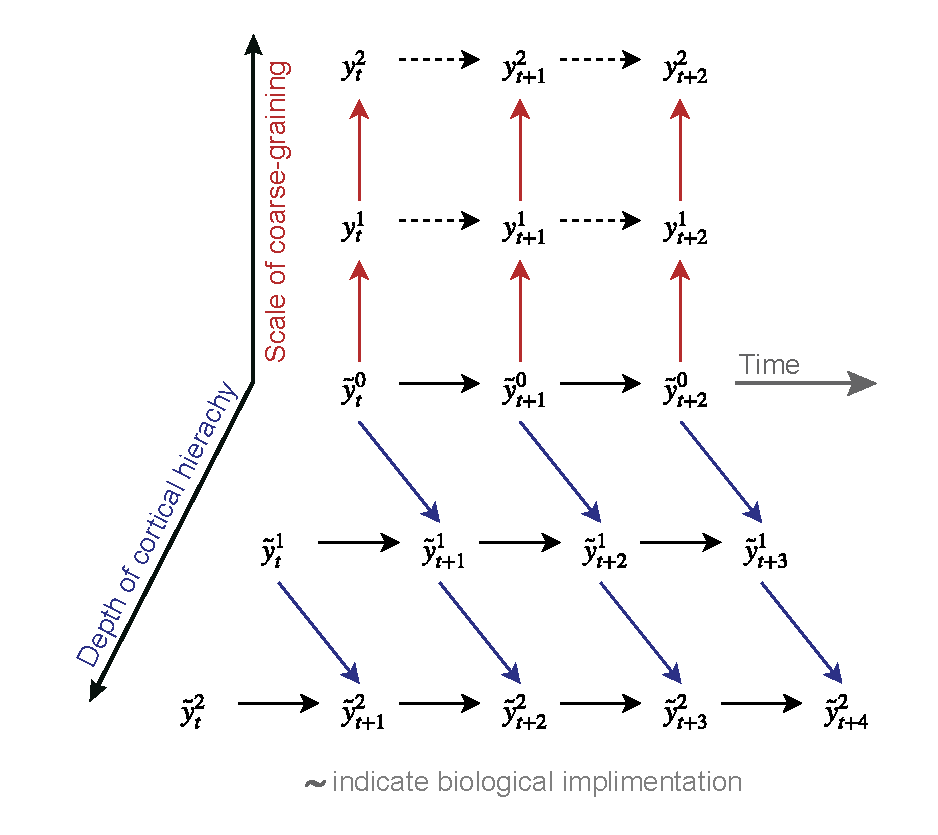
\includegraphics[width=\textwidth]{WritingMaterials/Fig_SeperationOfCGandCortHierachy/SeperationOfCGandCortHierachy.pdf}
				\caption{The distinction between the level of coarse-graining and the level of the cortical hierarchy. $X$ and $Y$ represent the microscopic and macroscopic coarse-grained  variables, respectively. $X^0$ represents the microscopic states at the upstream of the cortical hierarchy. The red empty arrows represents the directions of coarse-graining and the blue arrows represent the directions of the physical dependencies in the cortical hierarchy from the upstream to the downstream. (Some variables and dependencies are omitted for clarity.)}
				\label{fig:hierarchy}
    		\end{figure} 
    		
        
        % ---------------------------------------------------------------------------- %
        %                                      IIT                                     %
        % ---------------------------------------------------------------------------- %
		\subsection{Integrated Information Theory}
            Integrated information theory (IIT) states that consciousness is integrated information and system's consciousness is determined by its causal properties \citep{tononi2016integrated}. \ac{OurTheory} is in line with IIT in that informational properties are thought to underlie consciousness. In this section, we will discuss \ac{OurTheory} in the light of IIT. 
            
            \textbf{The concept of "information"}: In IIT, information refers to "integrated information":\\ \textquote[\citealt{tononi2016integrated}]{Information that is specified by a system that is irreducible to that specified by its parts.} In \ac{OurTheory}, information refers to "self-information", i.e. information about the states of conscious experience and the physical states of a process. Therefore, IIT focuses more on the relationships between consciousness and causal interactions among elements within a system, whereas \ac{OurTheory} focuses more on the informational relationships between conscious experience and being in a certain state of a process. 
		    
		    \textbf{The "Exclusion" axiom in IIT}: In IIT, the Exclusion axiom claims that of all overlapping sets of elements, only one set with maximal integrated information can be conscious. The exclusion axiom should be applied over elements, space, time, and scales \citep{oizumi2014phenomenology, hoel2016can}. \linelabel{line:multi-consciousness}Different from IIT, \ac{OurTheory} allows multiple consciousnesses coexist across different levels of coarse-graining within a system if they are informationally closed from each other. The two distinctive predictions decisively pinpoint the core concepts of the two theories. 

		    \textbf{The concept of "integration"}: In IIT, integrated information is one of the core concept of defining conscious individuals. In the current paper, we did not include the notion of integrated information within \ac{OurTheory}. This, however, results in one of the current weaknesses of \ac{OurTheory} that it lacks the ability to individuate NTIC processes in some extreme cases (i.e., the problem of individuality). We discussed this weaknesses in Sec.~\ref{sec:Limitation and Future work}.
		    
		    \textbf{Prediction after system damaged}:\linelabel{line:r2-cutting} \ac{OurTheory} and IIT lead to different predictions when a system suffers from a damage. For example, considering a densely connected networks whose dynamics forms an NTIC process. If we cut the network in half, IIT would predict that this results in two consciousnesses because elements in both networks still maintain high degrees of interactions. In contrast, \ac{OurTheory} would predict that this operation could completely destroy NTIC rendering both parts unconscious.
		    

        % ---------------------------------------------------------------------------- %
        %                            Predictive Processing                             %
        % ---------------------------------------------------------------------------- %
		\subsection{Predictive Processing}
    		Predictive processing (PP) is a powerful framework which integrates several ideas from neuroscience. This emerging theoretical framework posits that neural systems constantly generate predictions about incoming sensory signals and updates predictions based on prediction errors between predictions and sensory signals. According to PP, neural systems constantly perform unconscious statistical inference about hidden causes in the external environment. The perceptual contents are the "best guess" about the environment states including these hidden causes \citep{clark_2013, Hohwy2013}. PP is well integrated with Bayesian brain hypothesis and has been used to interpret conscious perception in many domains \citep{Hohwy2013, seth2014predictive}.
    		
    		%% The gaps between pp and consciousness
    		PP is a powerful explanatory framework for diverse brain functions. However, to serve as a theory of consciousness, PP is still incomplete due to two explanatory gaps. First, it has been known that the neural system is equipped multiple predictive mechanisms. Apparently, not all the predictive mechanisms are involved in conscious processes (e.g. mismatch negativity, \cite{naatanen2007mismatch}). PP needs to explain the difference between conscious and unconscious predictive mechanisms. 
    		
    		Second, PP can be considered as a sophisticated computation for perceptual inference. It takes von Helmholtz's conception of perception as unconscious inference. Thus, only the most probable outcome computed by the inference processes can be conscious while other details of the computation remain unconscious. PP also needs to explain how unconscious inferences is able to give rise to conscious results. In short, while PP is often discussed in the context of consciousness, these explanatory gaps prevent PP from being a theory of consciousness. 
    		
    		% compatible things
    		\ac{OurTheory} is well compatible with PP. Crucially, \ac{OurTheory} further provides natural and fundamental explanations to fills the two explanatory gaps which PP encounters. According to the definition of NTIC, a process with high NTIC can be regarded as a powerful predictive machine which has accurate self-predictive information ($I(Y_{t+1};Y_{t})$, E.q.~\ref{eq:NTIC1}) and concurrently incorporates environmental information into its dynamic ($I(Y_{t+1};Y_{t}|E_{t})$, E.q.~\ref{eq:NTIC1}). This predictive nature of NTIC processes is in agreement with the core notion of PP in which the conscious contents are always the predicted (inferred) outcome of our predictive mechanisms. Second, due to the informational closure to the environment, the encoded information about its environment in an NTIC process can be seemed as "the best guess" about the external environment in the context of Bayesian inference. 
    		
    		% fill the gaps
    		So, eventually, why are some predictive information conscious and some are not? \ac{OurTheory} predicts that only the predictions generated from mechanisms involving the NTIC process are conscious. Note that predictive processes are not necessary to involve NTIC processes. A predictive process can make prediction about the future state of its environment based on the current sensory inputs. In this case, the the process is not informationally closed and could not be conscious.
    		
            According to \ac{OurTheory}, we further propose that we can only be aware of the predictions from predictive processes due to informational closure to computational details of microscopic predictive processes. The macroscopic NTIC process only acquires the coarse-grained summary statistics of the microscopic processes. In other words, we predict that the computation of the statistical inferences of PP is implemented at microscopic (cellular) levels in the neural system. 
        
    		% finally
    		Finally, we consider PP as an potential empirical implementation of NTIC processes. To maintain accurate information about the environment encoded in an NTIC process, one can open an information channel between the process and the environment for minimal information flow to correct the divergence between them. This proposal is compatible with PP which suggests that PP systems updates (corrects) the current estimations by computing prediction errors between predicted and real sensory inputs. 


        % ---------------------------------------------------------------------------- %
        %                           Sensorimotor contingency                           %
        % ---------------------------------------------------------------------------- %
		\subsection{Sensorimotor Contingency}
    		Sensorimotor contingency (SMC) theory of consciousness proposes that different types of SMCs give rise to different characteristics of conscious experience \citep{o2001sensorimotor}. The theory radically rejects the view that conscious content is associated with internal representations of a system. Rather, the quality of conscious experience depends on agents' mastery of SMCs. SMC emphasises that the interaction between a system and its environment determines conscious experience. 
    	
    	    \ac{OurTheory} is not compatible with SMC. As mentioned in Sec.~\ref{sec:Conscious versus Unconscious Processing}, a process directly maps the sensory states to the action states is insufficient to be NTIC. Therefore, learning contingencies between sensory inputs and action outputs does not imply NTIC. Hence, \ac{OurTheory} predicts that having sensorimotor contingencies is neither a necessary nor a sufficient condition for consciousness. In fact, empirically, with extensive training on a sensorimotor task with a fixed contingency, the task can be gradually performed unconsciously. This indicates that strong SMCs do not contribute conscious contents. In contrast, \ac{OurTheory} suggests that, with extensive training, the neural system establishes a neural mapping from sensory inputs to action outputs. This decrease the level of informational closure and, as a result, decrease the conscious level of this process. This outcome strongly supports \ac{OurTheory} than SMC. 
    	    
    	    Nevertheless, \ac{OurTheory} does appreciate the notion that interactions between a process and its environment is crucial to shape conscious experience. As mentioned above, to form NTIC, a process needs to encode environmental transitions into its own dynamic. Therefore, information of agent-environment interaction should also be encoded in the NTIC process, and therefore, shape conscious contents in a specific way. 
    	    
    	    Different from the classical SMC, a new version of SMC, Predictive Processing of SensoriMotor Contingencies (PPSMC), proposed by \cite{seth2014predictive, seth2015presence} combines SMC and the predictive processing framework together. PPSMC emphasises the important role of generative models in computing counterfactuals, inferring hidden causes of sensory signals, and linking fictive sensory signals to possible actions. According to \ac{OurTheory}, if the generative model involving the NTIC process for the computation of counterfactuals, PPSMC will be compatible to our theory and may have strong explanatory power on some specific conscious experience.
    	    
				
        % ---------------------------------------------------------------------------- %
        %                            Global workspace theory                           %
        % ---------------------------------------------------------------------------- %
        
		\subsection{Global Workspace Theory}
		Global workspace theory (GWT; \cite{baars1988cognitive, baars1997theatre, baars2002conscious}) or Global Neuronal Workspace theory (GNWT; \cite{dehaene1998neuronal, dehaene2001towards, dehaene2011experimental}) states that the neural system consists of several specialised modules and a central global workspace (GW) which integrates and broadcasts information gathered from those specialised modules. Only the information in the global workspace reaches conscious awareness, and information outside of it remains unconscious. These modules compete with each other to gain the access to the GW and the information from the winner triggers an all-or-none "ignition" in the GW. Information in the GW is broadcasted to other modules. Conscious contents then are associates with the information that gains access to the internal global workspace \cite{Dehaene2017}.
		
        While GWT emphasises the importance of global information sharing as a basis of consciousness, the precise meaning of information broadcasting has been somewhat unclear if one tries to describe it more formally in the language of information theory. \ac{OurTheory} offers one possible way to consider the meaning of broadcasting in GWT. Specifically, one could interpret the global workspace as the network of nodes where information is shared at the scale of NTIC where communication is performed through macro-variables that are linked via mutual predictability. That is, global workspace should be also NTIC. While this link remains speculative at this point, this interpretation encourages empirical studies into the relationship between the contents of consciousness and macrostate neural activities that are mutually predictive of each other. 
		

% ============================================================================ %
%                                  Limitation                                  %
% ============================================================================ %
    \section{Limitation and Future Work}\label{sec:Limitation and Future work}  
        As a brand new theory of consciousness, \ac{OurTheory} is still far from completion. In the following, we discuss the current limitations and challenges of \ac{OurTheory} and point out the potential future research directions.
    
        % =============================== Theoretical  ===============================
        
        % Can't solve the hard problem
        It's important to clarify that \ac{OurTheory} does not intend to completely solve the hard problems of consciousness \citep{chalmers1995facing}. Knowing the state of a conscious process does not allow us to answer "What is it like to be in this state of this process" \citep{nagel1974like}. Instead, \ac{OurTheory} focuses more on bridging consciousness and the physical world using information theory as a common language in between.
        
        % Identity problem
        \linelabel{line:individuality}The current version of \ac{OurTheory} cannot entirely solve the problem of individuality in some extreme circumstances. In common cases, one can identify individual consciousnesses by computing the levels of NTIC of a process. This approach can also be applied to finding the boundaries of individual consciousnesses (for details of the boundary detection procedure, see \cite{krakauer2014information}). However, in some specific circumstances, individuality of consciousness is not clear. For instance, we can define a new process $Y$ and also its environment $E$ by recruiting two independent NTIC processes $Y^1~\&~Y^2$ and their environments $E^1~\&~E^2$, respectively. So that $Y = \{Y^1,Y^2\}$ and $E=\{E^1,E^2\}$. In such case, the new process $Y$ will also be NTIC to $E$. Therefore, the current version of \ac{OurTheory} cannot determine whether there are two smaller consciousnesses or one bigger consciousness (or 3 coexisting consciousnesses). The problem of individuality is a significant theoretical weakness of the current version of \ac{OurTheory}. The notion of integration is a possible remedy for this issue and we will address this issue more explicitly in our future work using the concept of synergy.
        
        % About the environment
        The current version of \ac{OurTheory} assume that consciousness is only contributed by non-trivial rather than trivial information encoded in a process. In other words, how much information about environmental states and dynamics encoded in a process is a key quantity for consciousness. However, we do not exclude the possibility that environmental information may be just a proxy of other informational quantities. More theoretical work is needed to elucidate the role of environments. This issue will also be discuss in our next theoretical paper. 
        
        \linelabel{line:dream}Explaining conscious experience during dreaming is always a challenge to all the theories of consciousness. ICT currently does not have a certain answer to dreaming. However, we want to emphasise that not all the processes in the neural system are NTIC. This is trivial since some processes are evidently not informationally closed. They mainly passively react to sensory inputs or other processes in the neural system. To the conscious (NTIC) process, the rest of the neural system is part of the environment, and undoubtedly retains some degree of activity during sleep and dreaming. We speculate that, during dreaming, the neural system stably forms an NTIC process with respect to its environment, i.e. the other parts of the neural system. However, at the current stage, this is mere speculation. Searching for the NTIC process(es) during dreaming is a crucial step to extend the scope of ICT in future research. 
        
        % ================================= Empirical ================================ 
        % finding the coarse-graining function 
        Empirically, a major challenge to \ac{OurTheory} is to find proper coarse-graining functions which map microscopic processes to macroscopic NTIC processes. This will become an imperative issue of finding neurological supporting evidence for \ac{OurTheory}. To find proper coarse-graining functions among infinite candidates \citep{price2007causation} seem to be very challenging. Nevertheless, there are still theoretical and technical progresses recently that may contribute to  solving this issue. For example, the concept of \textit{causal emergence} proposed by Hoel \citep{Hoel19790, Hoel2018} has been further developed recently. Causal emergence is highly relevant to the relationship between informational closure and coarse-graining. In their new study by \cite{klein2019uncertainty}, they started to compare how different coarse-graining functions influence causal emergence at macroscopic levels. \cite{PFANTE.2014, PFANTE.2014b} provides thorough mathematical analyses on level identification including informational closure. In neuroscience, the understanding of neural population codes also achieves a tremendous progress due to the advancement of recording technique and data science \citep{Kohn2016, panzeri2015neural}. \cite{Gamez2016} has also systematically described relevant issues in terms of finding data correlates of consciousness amount different levels of abstraction. We believe that interdisciplinary research is required to narrow down the scope of searching the coarse-graining functions and conscious processes at the coarse-grained levels in the neural system and beyond. 
        
        \linelabel{line:r1-state-dep}In this article, we do not use a state-dependent formulation of NTIC. However, we believe that the state-dependent NTIC is essential to describe the dynamics of conscious experience. Therefore, further research using point-wise informational measures to construct state-dependent NTIC is needed in the next version of ICT.
        
        Finally another empirical challenge to \ac{OurTheory} is the  of empirical supporting evidence. This is understandable because the concept of NTIC is relatively new in the history of information science, not to mention in neuroscience. Very few experiments and data collections are designed for examining NTIC properties in neural systems. To our knowledge, only two studies \citep{Palmer2015, sederberg2018learning} coincidentally examine relevant properties in salamander retina. They found that the a large group of neural populations of retinal ganglion cells encoded predictive information about external stimuli also had high self-predictive information about their own future states. This result is in line with the characteristic of NTIC. We expect that there will be more empirical studies examining relevant neural properties of NTIC. 

% ============================================================================ %
%                                  Conclusion                                  %
% ============================================================================ %
    \section{Conclusions}
    % short re-introduction 
    In this paper, we introduced \textbf{\acf{OurTheory}}, a new informational theory of consciousness. \ac{OurTheory} proposes that a process which forms \textbf{non-trivial informational closure (NTIC)} is conscious and through coarse-graining the neural system can form NTIC processes, i.e., conscious processes, at a certain macroscopic level. \ac{OurTheory} considers that information is a common language to bridge the gap between conscious experience and the physical reality. Using information theory, \ac{OurTheory} proposes computational definitions for both conscious level and conscious content. This makes \ac{OurTheory} be able to generalise to any system beyond the human brains. 
    
    % For neuroscience
    \ac{OurTheory} provides explanation for various findings from research of conscious and unconscious processing. The implications of \ac{OurTheory} point out that the levels of coarse-graining play a critical role in searching for neural substrates of consciousness. Improper measurements, e.g., too fine or too coarse in terms of the scale of measurements, of neurophysiological signals may lead to misleading results and misinterpretations. 
    
    
    % For scientific theory of consciousness
    \ac{OurTheory} reconciles several theories of consciousness. \ac{OurTheory} indicates that they conditionally coincide with \ac{OurTheory}'s implications and predictions but, however, not the fundamental and sufficient conditions for consciousness. For example, theories includes the theories emphasising recurrent circuits \citep{lamme2006towards, edelman1992bright}, the theories highlighting the internal simulation,  predictive mechanism, and generative models ~\citep{revonsuo2006inner, clark_2013,Hohwy2013, kanai_chang_yu_de_abril_biehl_guttenberg_2019, seth2014predictive, seth2015presence}, and theories related to multilevel view of consciousness~\citep{pennartz2018consciousness,pennartz2015brain,prinz2007intermediate, jackendoff1987consciousness}. Notably, \ac{OurTheory} is proposed based on the non-functional hypothesis. Notwithstanding, its implications for the functional aspects of a system well fit several functionalist proposals.
	
	
	% For philosophy of mind
	Regarding philosophy of mind, \ac{OurTheory} connects several distinct arguments together. \ac{OurTheory} can be seen as an identity theory because it assumes a fundamental relation between consciousness and information. Second, the implications of \ac{OurTheory} tightly link consciousness to several cognitive functions in the context of evolution. This explains why people might intuitively have a functionalist point of view of consciousness. \ac{OurTheory} emphasises that informational closure between levels of coarse-graining is critical to form NTIC processes in some stochastic systems. In this case, especially for the neural system, forming conscious processes at the macroscopic levels coincide with the perspective of emergentism. Finally, forming NTIC (conscious) processes through many-to-one maps, i.e., coarse-graining, implies multiple realisability of consciousness. As a result, \ac{OurTheory} provides an integrated view for these arguments and is further capable of indicating how and why they are conditionally true.
	
	% Final 
	So far, the current version of \ac{OurTheory} is still far from completion. Further theoretical and empirical research is indispensably required for \ac{OurTheory} to improve and solve several issues in the current version. Nevertheless, \ac{OurTheory} offers explanation and prediction for consciousness science. We hope that \ac{OurTheory} provides a new way of thinking and understanding neural substrates of consciousness.  
	
	% ============================================================================ %
	%                                      End                                     %
	% ============================================================================ %
	\section*{Acknowledgements}
	\addcontentsline{toc}{section}{Acknowledgements}
	A.C., Y.Y, and R.K. are funded by Japan Science and Technology Agency (JST) CREST project. Work by M.B. and R.K. on this publication was made possible through the support of a grant from Templeton World Charity Foundation, Inc. The opinions expressed in this publication are those of the authors and do not necessarily reflect the views of Templeton World Charity Foundation, Inc. This manuscript has been released as a Pre-Print at arXiv \citep{chang2019information}.


    \section*{Author Contributions Statement}
    \addcontentsline{toc}{section}{Author Contributions Statement}
    A.C. conceived and developed the theory. M.B. and A.C. contributed the mathematical formalisation of the theory. A.C., M.B, and R.K wrote the manuscript, based on a first draft by A.C. with extensive comments from Y.Y. All authors contributed to manuscript revision, read and approved the submitted version.

    \section*{Conflict of Interest Statement}
    \addcontentsline{toc}{section}{Conflict of Interest Statement}
    All authors were was employed by the company Araya Inc. The authors declare that the research was conducted in the absence of any commercial or financial relationships that could be construed as a potential conflict of interest.





	\bibliographystyle{authordate1}
	\addcontentsline{toc}{section}{Reference}
	\bibliography{ref}
	
	\section*{Figure Legends}
	\renewcommand{\listfigurename}{~}
	\addcontentsline{toc}{section}{Figure Legends}
    \listoffigures

\end{document}

\documentclass[utf8]{article}
% \usepackage{RevisionToolsByAcer}
% \ProvidesPackage{RevisionToolsByAcer}
% \documentclass[utf8]{article}
% \ProvidesPackage{RevisionToolsByAcer}
%% Language and font encoding
\usepackage[english]{babel}
\usepackage[round, sort]{natbib}
\usepackage[T1]{fontenc}



% ============================ Sourcing main file ============================ %
\usepackage{xr}
\externaldocument{ICT_Frontiers_rev202001}
\usepackage{lineno}





% Sets page size and margins
% \usepackage[a4paper, top=3cm,bottom=2cm,left=3cm,right=3cm,marginparwidth=4cm]{geometry}
\usepackage[papersize={10in, 12in}, top=3cm,bottom=2cm,left=2in,right=2in,marginparwidth=1.8in]{geometry}
\usepackage{titlesec}
\usepackage[dvipsnames,table,xcdraw]{xcolor}
\usepackage[at]{easylist}
\usepackage[round]{natbib}
\usepackage{amsmath}
\usepackage{graphicx}
\usepackage[colorlinks=true, allcolors=blue]{hyperref}
\usepackage{authblk}
\usepackage{float}
\usepackage{tikz}
\usepackage[threshold=2, autopunct=true, autostyle=true]{csquotes}
\usepackage[colorinlistoftodos]{todonotes}


% =============================== Header style =============================== %
\titlelabel{}


% ============================================================================ %
%                               Macros from Acer                               %
% ============================================================================ %

		
% --------------------------------- Question --------------------------------- %	
\newcounter{cQuestion}[section]
\newenvironment{question}
    {\refstepcounter{cQuestion}\color{Blue}\noindent\newline Q\thecQuestion:}
    {~\newline}
    
% ------------------------------------ Ans ----------------------------------- %
\newenvironment{ans}  
    {\color{Black}\noindent A:}
    {~\newline}    
    
    
\newcommand{\QA}[2]{
    \begin{question}  
        #1
    \end{question}
        
    \begin{ans}  
        #2
    \end{ans}
}

% ---------------------------------- Revise ---------------------------------- %
% \Revise{Page}{original text}{revised text}
\newcommand{\revise}[3]{
	\newline
	\newline
    \noindent
    \textbf{Line #1:}
    \newline
    Original:\newline
    \textit{"#2"}
    \newline
    \newline
    Revised:\newline
    \textit{"#3"}\newline}

% ---------------------------------- Add New --------------------------------- %
% \addnew{line number}{text}
\newcommand{\addnew}[2]{\blockcquote{}{\textbf{Line #1:}~\newline\textit{"#2"}}
}

% ================================ Annotation ================================ %
\newcommand{\toWrite}[1]{\noindent
	\textcolor{Orange}{\textbf{[[ #1 ]]}}}


% =================================== Title ================================== %
\title{Response to Reviewers $Rev^1$}
\date{\today}
\author{} 



% =================================== Begin ================================== % 
\begin{document}

    \maketitle
    \section*{Reply to Editor}
        \begin{question}
        In addition, I have a question. if we view molecules as coarse grains of elementary particles, would the phenomenon of molecular recognition have high NTIC and thus be conscious?
        \end{question}
        
        \begin{ans}
            Hi Prof. Hoffman,
            Thank you for your attention to our manuscript and your interesting question. \\
            There is no question that molecular complexes are coarse-grainings of molecules via molecular recognition. Based on our hypothesis, if the dynamics of a molecular complex is an NTIC process, the information closure theory of consciousness (ICT) would claim that the molecular complex has a certain degree of consciousness. Therefore, to your question, it is theoretically plausible under the framework of ICT. We speculate that it may be easy to find informationally closed molecular complexes (isolated complexes) but may not be easy to find ones forming NTIC processes. Nevertheless, with well-defined mathematical definition, this is an empirical and testable question to ICT. We look forward to learning any self-assembly process forming NTIC at molecular scales in the near future.        
        \end{ans}
        
    
    \section{Reply to Reviewer 1}
        \begin{question}
            Regarding the NTCI measure: \\\\
            a) Bertschinger et al. 2006 define informationally closed as $J_t(E -> Y) = 0$, but this is not a requirement for NTIC. Meaning, a positive NTIC measure does not entail that $J_t = 0$. $J_t = 0$ is only true if the NTIC is equal to $I(Y_{t+1}; E_t)$. In what sense does it correspond to non-trivial information closure then? (see also my concern \#2, maybe that is related) As defined in eq. 6 a video camera might have very high NTIC if it records a natural scene, even though it is in no way informationally closed from the environment.\\\\
            b) Is $NTIC_t$ state dependent or not? As capital letters are used I assume it is based on (conditional) mutual information measures across one time step but averaged over the possible states of the system at time t and t+1, so state distributions. But which distributions are used to compute $NTIC_t$? The stationary joint distribution of states at t and t+1? It cannot be just some observed measure, because then the level of consciousness would depend on how long the observation is. Moreover, if $NTIC_t$ is not state dependent, then the Reflex example on p. 10 is not intuitive. Because the system (brain) is the same and awake whether it behaves reflexively or not, so while the content may depend on the type of action, the $NTIC_t$ (level) would stay the same.              
        \end{question}
    
    	\begin{ans}
    		\newline
    		a) Considering Eq.\ref{eq:NTIC2}, it is true that the transfer entropy term $J_t(E -> Y)=0$ is not required for $NTIC>0$. It is possible to have a high degree of NTIC when $J_t(E -> Y) > 0$, i.e. the process is not completely closed.  \\
    		However, based on the setting in both Bertschinger et al. 2006 and our Section 2 (at Line \lineref{line:r1q1a}), $Y_{t+1}$ is determined by both $Y_t$ and $E_t$. Simply increasing $I(Y_{t+1}; E_t)$ without closedness (e.g, copy the information in sensory signals to the process such as the case in the video camera example), the transfer entropy term $J_t(E -> Y)$ should increase at the same rate and cancel out the increment of $I(Y_{t+1}; E_t)$ resulting low NTIC. Namely, keeping high closedness, i.e. minimising $J_t(E -> Y)$, is crucial to increase NTIC even though $J_t(E -> Y) > 0$.\\
    		In our current version of ICT, we consider the level of consciousness corresponds to the degree of NTIC of a process. Therefore, a conscious process does not have to be completely closed. However, a high degree of closedness is crucial to have a high level of consciousness.\\
    		
    		\noindent
    		b) Thank the reviewer for this outstanding question. We entirely agree that state-dependent measurements are essential to describe the dynamics of conscious experience. In fact, we now are working on state-dependent formulations for the next version of the ICT. In contrast to the current version, this work involves point-wise informational measures and certainly require more space and discussion. Therefore, we prefer to address the state-dependent version of ICT in future studies and keep the first version of our theory simple.\\
    		We appreciated that the reviewer pointed this out. We have added a short paragraph about this issue.
    	
	    	\addnew{\lineref{line:r1-state-dep}}{
	    		In this article, we do not use a state-dependent formulation of NTIC in the current version of ICT. However, we believe that the state-dependent NTIC is essential to describe the dynamics of conscious experience. Therefore, further research using point-wise informational measures to construct state-dependent NTIC is needed in the next version of ICT.}
	    	
	    		
	    		
    	\end{ans}
        
       
        
        \begin{question}
            Hypothesis and Implication 3: Why is it crucial that there is an underlying X with respect to which Y is a C-process? Does Y being informationally closed with respect to X imply that Y is also informationally closed with respect to E, i.e. $J_t(E-Y) = 0$? I don't think that could be true for the brain, or part of it really. My brain's next state, at whatever level, certainly depends to some degree on unpredictable sensory inputs from the environment. In the end, is $I(Y_{t+1}; E_t|Y_t) = 0$ required for consciousness or not? (see point 1a). In other points in the manuscript this does not seem required, e.g. p. 10 "If a process is not informationally closed, the degree of NTIC is low resulting in low or no consciousness".        
        \end{question}
        
        \begin{ans}        	
            Because X is the micro-level of the universe, any coarse-graining of X (including E and S) should have equal or less information about Y than X, i.e. $I(Y_{t+1}; X_t|Y_t) \geq I(Y_{t+1}; S_t|Y_t)$ and  $I(Y_{t+1}; X_t|Y_t) \geq I(Y_{t+1}; E_t|Y_t)$. Therefoe, Y is informationally closed with respect to X implying that Y is also informationally closed with respect to S, E, and all other coarse-grainings of X. As explained in Question 1a, it is not required for NTIC processes to be completely closed. Therefore, the closedness of Y with respect to X $I(Y_{t+1}; X_t|Y_t)$ serves as the lower bound of the closedness of Y to any other processes. 
            For this first exposure of our theory, we did not discuss NTIC in the context of the temporal coarse-graining. It is true that we certainly encounter some degree on unpredictable sensory inputs from the environment from time to time. Therefore, NTIC should be higher for finer temporal scales than for coarser temporal scales. We also speculate that the temporal coarse-graining is related to the speed of "stream of consciousness" and will address this issue in our future studies. 
        \end{ans}
        
        
        \begin{question}
            Exclusion or no exclusion? The authors state multiple times that "every process with a positive non-trivial information closure (NTCI) has consciousness." (p.3, and also p.12).
            a) Yet, Figure 4 is ambiguous in the sense that the maximum somehow seems important, while actually all levels should give rise to separate experiences. I don't see how ICT without something like exclusion (IIT style) would indicate that the maximum should correspond to human consciousness. It could just be any one out of many consciousnesses.
            b) p. 14: comparison to IIT: what does ICT say about different sets of variables at the same level. There might well be multiple ways to partition X into S and E, with many overlapping S's. Would those all be conscious? They would not be informationally closed from each other but they could all fulfill the requirements in the Hypothesis. It seems like finding the maximum within a level over the possible sets of elements/variables is a necessary step to identify boundaries (I think also Krakauer does that across sets of variables, but not 100\% sure)        
        \end{question}
    
    	\begin{ans}
			We do not impose the exclusion criterion in ICT. Instead, the concept of informational closure already involved the notion of individuality and was used to identify the system-environment distinction \citep{BERTSCHINGER.2006} and level identification \citep{PFANTE.2014} in system theory (however not complete, please see our discussion at Line \lineref{line:individuality}). In \cite{BERTSCHINGER.2006},
			
			It is true that if we assume a process $Y$ is NITC with respect to $E$. Every subset of $Y$ can have different degrees of NTIC with respect to $E$ as well. However, it is important to note that the subsets are not "other consciousnesses". Rather, they are subspaces of this conscious process $Y$.
			
			\toWrite{I this this is still bad}
			
%			\textit{If we sample a subset of elements, if its closedness is lower than 
%			Consider a simplified case, a process $Y$ is NITC with respect to $E$. 
%			For Any subset of 
%			A partition of $Y$ is a set $P_y$ which divides $Y$ into two subsets $P_y=\{Y_1, Y_2\}$. }    		    		    		
    	\end{ans}

        
        \begin{question}
            Feedback and memory: p. 11. If $NTIC > 0$ is sufficient and true information closure is not required, then feedfoward networks can be conscious according to ICT. Also, in that case, memory is not necessary, as the video camera would have $NTIC > 0$ as long as it records from a stable environment. In that case $I(Y_{t+1}, Y_t) > 0$ and $I(Y_{t+1}, Y_t|E_t)$ is small. This issue here is that having information about the next state does not imply that there is any causation, so if $Y_t$ is highly correlated with $E_t$ and $E_t$ causes $Y_{t+1}$ then NTIC is high. (Thus the IIT emphasis on causation).\\
            If somehow the fact that Y must be informationally closed wrt X does the heavy-lifting here that should be made more explicit (see above).
        \end{question}
        
        \begin{question}
            Does ICT imply that one is unconscious while dreaming? In that case $I(Y_{t+1}; Y_t|E)$ should almost be identical to $I(Y_{t+1};I_t)$ and thus lead to NTIC approx. 0.        
        \end{question}
    
    	\begin{ans}
	    	We want to emphasise that not all the processes in the neural system are NTIC processes. This is evident since some processes in the neural system are not informationally closed. They only passively react to sensory inputs or other processes of the neural system. 
	    	
	    	To the conscious (NTIC) process, the rest of the neural system is considered as part of the environment. This notion is shortly indicated at line \lineref{line:neu-env} in our original manuscript. There is no doubt that these processes are still active during sleep and dreaming. We speculate that, during dreaming, the neural system can stably form the NTIC process with respect to its environment, i.e. other parts of the neural system.  However, at the current stage, this is mere speculation so we restrained ourself from making the statement in our manuscript. However, we thank the reviewer for bringing up this important question. We believe that this is still worth mentioning. We have added a short paragraph as follows:
	    	
			\addnew{\lineref{line:dream}}{Explaining conscious experience during dreaming is always a challenge to all the theories of consciousness. ICT currently does not have a certain answer to dreaming. However, we want to emphasise that not all the processes in the neural system are NTIC. This is trivial since some processes are evidently not informationally closed. They mainly passively react to sensory inputs or other processes in the neural system. To the conscious (NTIC) process, the rest of the neural system is part of the environment, and undoubtedly retains some degree of activity during sleep and dreaming. We speculate that, during dreaming, the neural system stably forms an NTIC process with respect to its environment, i.e. the other parts of the neural system. However, at the current stage, this is mere speculation. Searching for the NTIC process(es) during dreaming is a crucial step to extend the scope of ICT in future research.}
	    	
	    	Finally, we believe that this is also an
	    	empirical question that can and should be tested in future studies.
    	\end{ans}
        
        
        \begin{question}
            Minor:
            \begin{enumerate}
                \item "contributions to the field" This section is just a copy paste from the abstract and thus not necessarily helpful. Not sure though what the purpose of this section is meant to be by Frontiers.
                
                \item Introduction: "We currently lack a theory... " IIT and the geometric theory of consciousness (Fekete et al.) have proposed solutions. So there are theories. The following paper should be of interest and should probably be cited:
                Fekete T, van Leeuwen C, Edelman S (2016) System, subsystem, hive: Boundary problems in computational theories of consciousness. Front Psychol 7:1041.
                
                \item $y_t$ corresponds to the content. I would argue that an activation state, without taking the system or relation between elements etc into account is meaningless and cannot capture/explain the structure of an experience. Though this issue can be dealt with at a later time.
            \end{enumerate}
        \end{question}
    
    	\begin{ans}
    		\begin{enumerate}
    			\item It's true that we were also confused about it during submission. 
    			We have modified this as follows: \\
    			\toWrite{"contributions to the field"}
    			
    			\item Thank the reviewer for the reminder. We have modified our manuscript and cited the relevant references. 
    			\revise{\lineref{line:lack-theory}}
    			{We currently lack a theory to identify the scale which conscious processes correspond to.}
    			{We currently have only few theories (e.g., Integrated Information Theory \citep{hoel2016can} and Geometric Theory of consciousness \citep{fekete2011towards,fekete2012lack}) to identify the scale which conscious processes correspond to (please also see the discussion in \cite{fekete2016system}).}    			
    			
    			\item We agree with the reviewer's comment. 
    			In fact, in ICT, we do not differentiate states of processes between activation and relation. Take neural networks as an example, activation and structure states of a neural network should be both considered. After all, they are all just parameters of the process of the neural network. The only difference between the two groups of the parameters is the temporal scales of the parameter changes. States of activation may have more rapid dynamics than states of relation. In ICT, this is crucially related to the coarse-graining at the temporal domain which we did not address in this article but can be easily generalised in the future versions of ICT. 
    			
    			\todo{Do we need to write something in the main text?}
    			
    			
    		\end{enumerate}
    		
    	\end{ans}
        
        
    \section{Reply to Reviewer 2}
        \begin{question}
			I had a few problems in reading the paper, which I think should be addressed (especially the first) before the paper is published. For detailed notes on these see below.
			
			\begin{enumerate}
				\item The coarse-graining idea seems undefined in critical ways, but the paper reads as though it is well-defined. So maybe the authors have compressed too much detail? In the formalism presented it is unclear what coarse-graining (or information closure to other grains) amounts to. With this lack of detail, it is then unclear to me why intermediate maxima in IC are a plausible result (why does IC not just decline with progressive coarse graining).
				
				\item The idea of 'simulation'. This is a more minor point but I would appreciate if the authors could be clearer on this. It is arguable whether or not consciousness simulates anything (e.g. see Hoffman's interface theory); and some of the assertions the authors make re simulation seem unfounded anyways. But it could be that they mean something different or subtle (that consciousness is linked to or represents or etc the environment)
				
				\item There were several other assertions that stood out to me as strange or wrong, but could be a matter of explanation or ignorance on my part (the feedforward system, the cut-apart system). Either way some more explanation would be good.
			\end{enumerate}
        \end{question}
    
    
    	\begin{ans}
    		\begin{enumerate}
    			\item In this article, the definition of coarse-graining is our "Definition 1" (line: \lineref{line:r2q1-1}). Coarse-graining is simply a function which maps a stochastic process $X$ with state space $\mathcal{X}$ to a stochastic process $Y$ with state space $\mathcal{Y}$. As we explained in Footnote 2, functions in the mathematical sense used here are always either one-to-one or many-to-one. We do not constrain ICT to be applied to any specific classes of coarse-graining.
    			Thank the reviewer for proposing the question about the relationship between NTIC and scale of coarse-graining. We currently know that NTIC is not a non-monotonic function of the scale of coarse-graining. Some coarse-grainings lead to higher NTICs for macroscopic than microscopic processes. However, we are just starting the research on this relationship, and have not yet had a systematic understanding of it. This work may involve the technique of partial information decomposition and related research fields. 
    			We agree that our original claim about existing a intermediate maxima in NTIC was too strong. 
    			
    			
    			We hope to address this question in future research. 
    			
    			
    			
    			We emphasise the non-monotonic relation between the scales of coarse-graining and the degrees of NTIC. However, we do not exclude the possibility that there exist multiple NTIC picks across scales of coarse-graining of a process. 
    			This implies that we do not exclude the possibility that there exist multiple high conscious processes at different scales. 
    			(However, due to IC, conscious processes are not able to know the existence of each other. 
    			\revise{\lineref{line:non-monotonic}}
    			{
    				It is important to note that NTIC can be a non-monotonic function of the scale of coarse-graining. We saw above that not sufficiently coarse-grained variables have low values of NTIC. On the other hand, overly coarse-grained macroscopic variables  also result in low values of NTIC. For example, in an extreme scenario, when all microscopic states map to a single macroscopic variable, the macroscopic level does not have any information capacity and thus cannot have high mutual information across time steps. Therefore, only processes at a certain level of coarse-graining in the neural system can form a high degree of NTIC (Fig.~\ref{fig:LevelOfConsciousness}). ICT indicates that human consciousness occurs at the level of coarse-graining where higher NTIC is formed within the neural system.
    			}
    			{
    				It is important to note that NTIC can be a non-monotonic function of the scale of coarse-graining. Insufficiently coarse-grained variables could lead to lower values of NTICs at micro than macroscopic processes. On the other hand, overly coarse-grained macroscopic variables also result in low values of NTIC. For example, in an extreme scenario, when all microscopic states map to a single macroscopic variable, the macroscopic level does not have any information capacity and thus cannot have high mutual information across time steps. Therefore, processes at certain levels of coarse-graining may have higher values of NTIC than other levels (Fig.~\ref{fig:LevelOfConsciousness}). ICT suggests that human consciousness occurs at the level of coarse-graining where higher NTIC is formed within the neural system.
    			}										
    			\item \toWrite{TBD}
%    			\item \toWrite{After replying the first reviewer}
    		\end{enumerate}
    		
    	\end{ans}
    
    
    	
        
        
        \begin{question}
			The English is not perfect and needs some good proofreading, though it was understandable throughout.
        \end{question}
    
    
    	\begin{ans}
    		\todo{What should we deal with this?}
    	\end{ans}
    
    
    	\begin{question}
			On line 182, defining C-processes as cases where ‘Y is informationally closed to X’. This is now information closure in the sense of coarse-graining, but no such thing has been defined yet? Is it supposed to be so trivial that it is not required to make it explicit? To this point, closure is defined entirely in terms of system with respect to environment.
			
			Basically, I am not sure whether closer between scales is a matter of same-time (e.g. $I(Y_{t+1};X_{t+1})$) or across-time interactions ($I(Y_{t+1};X_t)$). Or could it be both?    		
    	\end{question}
    
    	\begin{ans}
			We followed a common setting of coarse-graining (e.g. \cite{PFANTE.2014}) which does not and should not take time $Y_t=f_Y(X_t)$ (in Definition 1). Coarse-graining is merely a function which maps microstates of a system to macrostates, and the microstates and the macrostates are simply different level of descriptions of a system. 
			Following this setting, the definition of information closure (flow) $J_{t}(X \rightarrow Y )$ can also be applied in the sense of coarse-graining. 
						
			We understand that this may lead to confusion for our readers. We have added the following sentence to make this point explicit.     		
			\addnew{\lineref{line:IC2CG}}{Note that we applied the same definition of information closure (Eq.\ref{eq:InformationFlow}) to processes at different coarse-grained levels \citep{{PFANTE.2014}}.}
%			Here, we followed a common setup of coarse-graining (e.g. \cite{PFANTE.2014}) which does not take time $Y_t=f_Y(X_t)$ (in Definition 1). In this setup, coarse-graining is unidirectional ad does not involve interaction between scales. This means that coarser scales supervene on finer scales, and there exists no top-down causation. \\
%			In our hypothesis, Y is IC with respect to the microstate of the universe, X. This is critical in the hypothesis because Y is IC with respect to X, implying that Y is also IC with respect to its intermediate level S and its environment E in Fig. \ref{fig:fullgraph}.\todo{need any change in the main text?}
    	\end{ans}
    
    
    	\begin{question}            
    		On line 241: “.. not sufficiently coarse-grained variables have low values of NTIC”, this is phrased as though it is necessarily true (and also that “we saw above”, though I do not see above where this is justified), but is it?
    		
    		At the very finest grain, wouldn’t even all the most ‘stochastic’ dynamics of a system be accounted for by prior states of the system, or by the environment? Why wouldn’t we assume that NTIC *only decreases* as the system is coarse-grained (as number of elements/states is decreased), for similar reasons as it must be zero at a 1-element 1-state system as the authors note? This seems an important point to be very clear on…
    	\end{question}
    
    	\begin{ans}
    		\toWrite{The reviewer is right?}
    		Thank the reviewer for this critical comment. It is true that NTIC a monotonic function of scales of coarse-graining. NTIC can increase or decrease when the grains are coarser. We are currently still working on the relationship between scales and NTIC. 
    		We will systematically address NTIC and functions of coarse-graining in our following studies. 
    		Further more, in our current analysis, it seems that this is also related to informational synergy and redundancy. We aim for presenting the core concept of ICT in this article.
    		The reviewer's critical question is on our list of future work. 
    		\toWrite{Need to change the text a lot!!}
    	\end{ans}
    
    
    	\begin{question}
    		on line 263: “NTIC processes encodes environmental information in its state. This suggests that a NTIC process can be considered as a process that simulates the environmental dynamics.“
    		
    		Why does encoding suggest simulation? An encoding *could* be a simulation, but it could well be nothing like a simulation, if we understand simulation to mean something like an imitation or reconstruction of some structure or dynamics. Two totally different environmental situations could potentially be encoded in exactly the same way (eg. as a string of 1s and 0s).
    		
    		The ‘simulation’ notion is brought up again in section 5.2 (line 344), citing Bertschinger et al, though I do not find the idea in that paper.. I think authors need to be clearer on what they mean by ‘simulation’ to make this point.
    	\end{question}
    
    	\begin{ans}
    		Thank the reviewer for this mindful comment. 
    		Our wording indeed is not clear. The notion of simulation is the same as the 'Modeling' case on Page 4 in \cite{BERTSCHINGER.2006}: 
    		\begin{quote}
		    	\textit{"B2)~Modeling: The system reaches synchronization and internalizes the correlations observed in the environment by building up own structures."}    	
    		\end{quote}    	
    	
    		To avoid the confusion We have revised the following sentence, changed "simulation" to "modeling", and added the reference.
    		\revise{\lineref{line:encode}}
    		{
    			Importantly, NTIC processes encode environmental information in its state. This suggests that a NTIC process can be considered as a process that simulates the environmental dynamics. }
    		{
    			Importantly, NTIC processes internalise the environmental dynamics in its states \citep[also see P.~4][]{BERTSCHINGER.2006}. This suggests that a NTIC process can be considered as a process that models the environmental dynamics.
    		}
    	\end{ans}
    
   	\begin{question}
			line 306: “Blindsight patients… make above chancel-level visual judgments without having any conscious perception about visual stimuli” I am not sure this characterization of blindsight is correct, it may be a matter of the phrasing. It could be - or probably is - the case that ‘blindsight’ patients always have some conscious experience of what drives their correct responses, but that the “visual character” of these experiences is degraded or missing.
			(Overgaard, Experimental Brain Research 2011)
			for a specific example
			(Mazzi, Bagattini, Savazzi; Frontiers in Psychology, 2016)
    	\end{question}
    
    
   		\begin{ans}
   			Thank the reviewer for the clarification. 
   			Yes, we specifically wanted to address the visual character of their experience. We agree that some patients still preserve some forms of conscious experience. 
   			We have changed our sentence and cited the relevant references as follows:
   			\revise{\lineref{line:r2q6}}
   			{
   				Blindsight patients are able to track objects, avoid obstacles, and make above chance-level visual judgements without having any conscious perception about visual stimuli.
   			}
   			{
   				Blindsight patients are able to track objects, avoid obstacles, and make above chance-level visual judgements with degraded or missing visual experience (however, in some cases, they may still preserve some forms of conscious experience, see \cite{overgaard2011visual, mazzi2016blind}). 
   			}
   		\end{ans}
    
    
    
    
    	\begin{question}
            on Line 316: On the issue of a feedforward network, the current state of a feedforward network with more than one layer is certainly driven by its own past states! So, mutual information of a feedforward network over a time lag should not be zero, unless I am misunderstanding something here?
			At the same time, I can see a version of the authors' argument here - for a unit in a feedforward network with depth (distance-from-input) of N, a time lag of N time steps would always account fully for the states of the element. Is this the idea?		
    	\end{question}
    
 		\begin{ans}
			Thank the reviewer for proposing this interesting and valuable comment. \\
			We can consider a simple case in which a feedforward neural network $Y$ consists of three layers, $Y^0$, $Y^1$, and $Y^2$. 
			$Y^0$ receives sensory input from the environment $E$. Each layer $Y^i_t$ passes information to the next layer $Y^{i+1}_{t+1}$ with a constant time cost $\Delta t$ as showed in the following figure.

 			\begin{figure}[H]
 				\centering
 				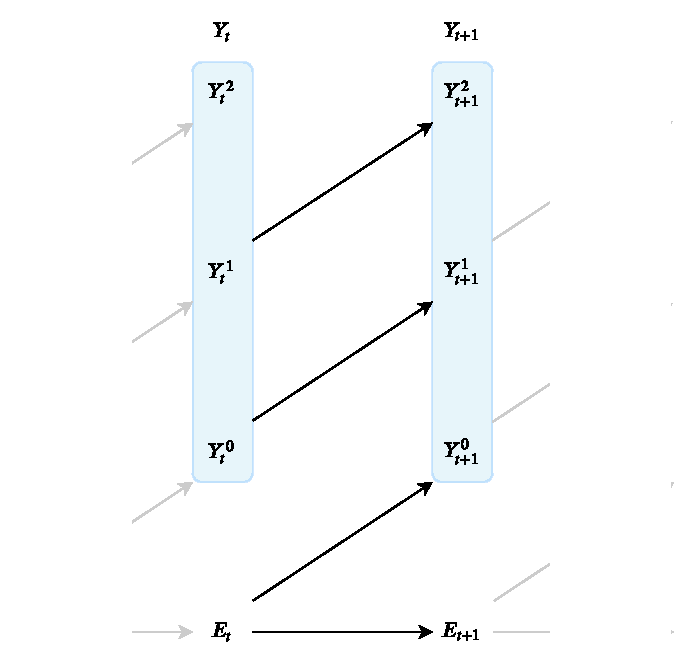
\includegraphics[width=\textwidth]{WritingMaterials/Fig_rev1_feedforward/Fig_rev1_feedforward} 				
 				\label{fig:rev1_feedforward}
 			\end{figure}
 			
			Because $Y^0_t$ determines $Y^1_{t+1}$ and $Y^1_t$ determines $Y^2_{t+1}$, it is true that the mutual information $I(Y_t; Y_{t+1}) \geq 0$. However, $E_t$ only influences $Y^0_{t+1}$ at time $t+1$. Therefore
			\begin{equation*}
				\begin{aligned}
					& I(Y_t; Y_{t+1}|E_t) = I(Y_t; Y_{t+1}) & \text{and} \\
					& NTIC_t(E\rightarrow Y)=I(Y_{t+1};Y_{t})-I(Y_{t+1};Y_{t}|E_{t}) =0  { }
				\end{aligned}
			\end{equation*}	
			
			Therefore, a feedforward network passively driven by input signals should have zero NTIC even though when time step (temporal coarse-graining) is small. 
			\todo{I don't think I answer this question well. Do we need to add anything in the main text?}
			 		
 		\end{ans}
 	
    
    	\begin{question}
    		on line 441: under the 'Prediction after system damaged', it is suggested that ICT predicts cutting a system in half would render both halves unconscious. But this would only be the case if neither half contains its own C-processes, yes? Since ICT allows that many C-processes can exist at the same time, it would have to be some special case for this prediction to hold true. So it seems to me the prediction is actually similar to that of IIT.
    	\end{question}
    
    
    	\begin{ans}
    		Thank the reviewer for this considerate comment. The reviewer is correct. This prediction is under an assumption which we did not explicitly specify in our last version. We assume that we have one conscious (NTIC) process involving information in both brain hemispheres. Namely, the process is informationally closed only when we consider the information in both hemispheres. We agree that if both hemispheres have their own NTIC proceess ICT should predict no change of conscious experience before and after cutting. Cutting should not make any difference because they are informationally closed with respect to each other. We also agree that this prediction is relatively premature. However, we also acknowledge the strength of all computational theories of consciousness. The reviewer's question is empirical to us under formal mathematical formulations of ICT and IIT. Systematical comparisons between model predictions can be done by rigorous modelling studies in the future. 
    		
    		\toWrite{The original paragraph has been changed as follows: lline \lineref{line:r2-cutting}:}
    	\end{ans}
    
                
        \begin{question}                                                                   
            Line 540: the theory doesn’t really seem to intend to solve the hard problem(s) at all, much less “completely solve”.            
            I was expecting the problem of dreaming to come up in the last section (maybe along with SMC for which it is a serious problem). When dreaming the information between environment and the system is virtually zero; is this a problem for ICT? Also, more specific phenomena like the eigengrau - if you take away all visual input, for long enough, I do not lose my visual experiences - rather they take on a special state. Does ITC need to accept the possibility that even *trivial* IC can be a conscious process?
        \end{question}
    
    	\begin{ans}
    		ICT is our first attempt to approach the hard problem of consciousness. We hope that ICT and our following works can establish an informational perspective on conscious experience. Instead of solving the hard problem of consciousness, we more look forward to mathematically determining whether the hard problem can be solved or not by information theory. However, because the relevant discussion is clearly outside the scope of this article, we prefer not to discuss the hard problem here.
    		
			We want to emphasise that not all the processes in the neural system are NTIC processes. This is evident since some processes in the neural system are not informationally closed. They only passively react to sensory inputs or other processes of the neural system. 

    		To the conscious (NTIC) process, the rest of the neural system is considered as part of the environment. This notion is shortly indicated at line \lineref{line:neu-env} in the original manuscript. There is no doubt that these processes are still active during sleep and dreaming. We speculate that, during dreaming, the neural system can stably form the NTIC process with respect to its environment, i.e. other parts of the neural system. The same idea can be also applied to phenomena like Eigengrau. However, at the current stage, this is mere speculation so we restrained ourself from making the statement in our last version of the manuscript. However, we thank the reviewer for bringing up this important question. We believe that this is still worth mentioning. We have added a short paragraph as follows:
    		
    		\addnew{\lineref{line:dream}}{Explaining conscious experience during dreaming is always a challenge to all the theories of consciousness. ICT currently does not have a certain answer to dreaming. However, we want to emphasise that not all the processes in the neural system are NTIC. This is trivial since some processes are evidently not informationally closed. They mainly passively react to sensory inputs or other processes in the neural system. To the conscious (NTIC) process, the rest of the neural system is part of the environment, and undoubtedly retains some degree of activity during sleep and dreaming. We speculate that, during dreaming, the neural system stably forms an NTIC process with respect to its environment, i.e. the other parts of the neural system. However, at the current stage, this is mere speculation. Searching for the NTIC process(es) during dreaming is a crucial step to extend the scope of ICT in future research.}
    		    
    		Finally, we believe that this is also an
    		empirical question that can and should be tested in future studies. 
    	\end{ans}

	\bibliography{ref}
\end{document}
